
% load packages
\documentclass[]{article}
\usepackage{amsmath,amssymb}
\usepackage{bm}
\usepackage{lmodern}
\usepackage{xcolor}
\usepackage{hyperref}
\usepackage{url}
\usepackage{parskip}
\usepackage{graphicx}
\usepackage{subfigure}

\title{Model-based Clustering for Neural Populations}
\author{}
\date{}
\begin{document}
\maketitle

The goal for this research is to do model-based clustering for  neural populations, by making use of features for each counting process observation. 

\section{Notations}

Assume we can observe neural activities for \(N\) neurons, with counting observation up to \(T\) steps. Therefore, the observation is a \textsl{N-by-T} matrix, \(\mathbf{Y} \in \mathbb{Z}_{\geq 0}^{N \times T}\) ,with each row represents the recording from single neuron. Denote the recording for neuron \(i\) as
\(\mathbf{y}_{i} = (y_{i1},\ldots,y_{\text{iT}})'\), \(i = 1,\ldots N.\), with the cluster index for neuron \(i\) as
\(z_{i} \in \{ 1,\ldots\}\). The number of neurons in cluster \(j\) is
\(n_{j} = \sum_{i = 1}^{N}{I(z_{i} = j)}\), and
\(\sum_{j = 1,2,\ldots}^{}n_{j} = N\). The proportion/ probability in
cluster \(z_{i}\) is \(\rho_{z_{i}}\).

\section{Clustering Wrapper}
The model-based clustering problem can be transformed into fitting the mixture model (MM). The likelihood for each cluster depends on how we model the counting observation, but fitting strategies for MM are the same for all models. Here, I choose to fit the MM by Gibbs sampler. Depending on whether the number of cluster is finite or not, there are two versions: finite mixture model (FMM) and Dirichlet process mixture model (DPMM).

\subsection{Finite Mixture Model}	
Assume the number of cluster is \(J\). The full likelihood for these \(N\) neurons is
\[L = \prod_{i = 1}^{N}{\rho_{z_{i}}f\left( \mathbf{y}_{i}|\mathbf{\Theta}_{z_{i}} \right)} = \prod_{j = 1}^{J}{\rho_{j}^{n_{j}}\left\lbrack \prod_{i:z_{i} = j}^{}{f\left( \mathbf{y}_{i}|\mathbf{\Theta}_{j} \right)} \right\rbrack}\]
, where \(\mathbf{\Theta}_{j}\) contains all parameters in cluster \(j\) defined by the specific model. Therefore, the parameters need to update are:
\begin{enumerate}
	\def\labelenumi{(\arabic{enumi})}
	\item
	Cluster indicator: \(\left\{ z_{i} \right\}_{i = 1}^{N}\)
	\item
	Cluster proportion: \(\mathbf{\rho} = (\rho_{1},\ldots\rho_{J})'\)
	\item
	Model parameters: \(\mathbf{\Theta}_{j}\)
\end{enumerate}
The (conditional) priors for clustering-related parameters:
\begin{enumerate}
	\def\labelenumi{(\arabic{enumi})}
	\item
	Cluster indicator \(\left\{ z_{i} \right\}_{i = 1}^{N}\):
	\(P\left( z_{i} = j \right) = \rho_{j}\)
	\item
	Cluster proportion \(\mathbf{\rho} = (\rho_{1},\ldots\rho_{J})'\):
	\[\mathbf{\rho} \sim Dir(\delta_{1},\ldots\delta_{J})\]
	, where \(\delta_{1} = \ldots = \delta_{J} = 1\)
\end{enumerate}

So, the MCMC( Gibbs sampler) iteration for FMM is:
\begin{enumerate}
	\def\labelenumi{(\arabic{enumi})}
	\item
	Update \(\left\{ z_{i} \right\}_{i = 1}^{N}\):
	\[P\left( z_{i} = j \middle| \mathbf{y}_{i},\left\{ \mathbf{\Theta}_{j} \right\}_{j = 1}^{J} \right) \propto \rho_{j}f\left( \mathbf{y}_{i}|\mathbf{\Theta}_{j} \right)\]
	\item
	Update \(\mathbf{\rho} = \left( \rho_{1},\ldots\rho_{J} \right)^{'}\):
	\[\mathbf{\rho}|\ \left\{ \mathbf{y}_{i} \right\}_{i = 1}^{N},\ \left\{ z_{i} \right\}_{i = 1}^{N},\left\{ \mathbf{\Theta}_{j} \right\}_{j = 1}^{J} \sim Dir(\delta_{1} + n_{1},\ldots\delta_{J} + n_{J})\]
	\item
	Update \(\mathbf{\Theta}_{j}\): this is defined by the specific model. When there's no
	\(z_{i} = j\), just sample \(\mathbf{\Theta}_{j}\) from priors or by other observation-independent ways.
\end{enumerate}

\subsection{Dirichlet Process Mixture Model}

Since calculation of posterior predictive distribution can be hard or even impossible for complicated models, instead of using the popular CRP representation of DP (Neal, 2020), I choose to use the slice sampler (\href{https://www.tandfonline.com/doi/full/10.1080/03610910601096262}{Walker, 2007}).

Use the ''stick-breaking'' construction for cluster proportion, i.e.
\[\rho_{1} = \eta_{1}\]
\[\rho_{j} = \left( 1 - \eta_{1} \right) \cdot \ldots \cdot \left( 1 - \eta_{j - 1} \right)\eta_{j}\]
\[\eta_{j} \sim Beta(1,\alpha)\]

In the slice sampler for DPMM, the parameters need to update are:
\begin{enumerate}
	\def\labelenumi{(\arabic{enumi})}
	\item
	``stick-breaking'' elements: \(\eta_{j}\)
	\item
	Augment latent variable: \(\left\{ u_{i} \right\}_{i = 1}^{N}\)
	\item
	Model parameters: \(\mathbf{\Theta}_{j}\)
	\item
	Cluster indicator: \(\left\{ z_{i} \right\}_{i = 1}^{N}\)
\end{enumerate}

So, the MCMC( Gibbs sampler) iteration for DPMM is:
\begin{enumerate}
	\def\labelenumi{(\arabic{enumi})}
	\item
	update \(\eta_{j}\), for
	\(j = 1,\ldots,{{z^{*} = max}\left\{ z_{i} \right\}}_{i = 1}^{N}\) as
	\[\eta_{j}|\left\{ z_{i} \right\}_{i = 1}^{N},\ldots \sim Beta(n_{j} + 1,\ N - \sum_{l = 1}^{j}n_{l} + \alpha)\]
	\item
	update \(\left\{ u_{i} \right\}_{i = 1}^{N}\):
	\[u_{i}|\mathbf{\rho,\ldots} \sim U(0,\ \rho_{z_{i}})\]
	\item
	update \(\eta_{j}\), for \(j = z^{*} + 1,\ldots,\ s^{*}\). \(s^{*}\)
	is the smallest value, s.t.
	\(\sum_{j = 1}^{s^{*}}\rho_{j} > 1 - \min{\{ u_{1},\ldots,u_{N}\}}\)
	\[\eta_{j} \sim Beta(1,\alpha)\]
	\item
	Update \(\mathbf{\Theta}_{j}\): this is defined by the specific model. When there's no
	\(z_{i} = j\), just sample \(\mathbf{\Theta}_{j}\) from priors or by other observation-independent ways.
	\item
	Update \(\left\{ z_{i} \right\}_{i = 1}^{N}\)
	\[P\left( z_{i} = j \middle| \mathbf{y}_{i},\left\{ \mathbf{\Theta}_{j} \right\},\mathbf{\rho,}\left\{ u_{i} \right\}_{i = 1}^{N} \right) = \frac{f\left( \mathbf{y}_{i}|\mathbf{\Theta}_{j} \right)}{\sum_{j:\rho_{j} > u_{i}}^{}{f\left( \mathbf{y}_{i}|\mathbf{\Theta}_{j} \right)}}\]
\end{enumerate}

\section{linear Dynamical System Model}
Here, I model the observations by a linear dynamical system (LDS) model.

LDS models the multi-dimensional time series using a lower dimensional latent representation of the system, which evolves over time according to linear dynamics. By specifying the linear dynamics and process noise covariance, we can also handle the interactions between different neural populations (clusters).

\subsection{Model Details}
Denote the latent vector in cluster \(j\) as
\(\mathbf{x}_{t}^{(j)} \in \mathbb{R}^{p_{j}}\). For simplicity, assume all \(p_{j} = p\). Each observation follows a Poisson distribution:
\[\log\lambda_{\text{it}} = d_{i} + \mathbf{c'}_{i}\mathbf{x}_{t}^{(z_{i})}\]
\[y_{\text{it}} \sim Poisson(\lambda_{\text{it}})\]
, where \(\mathbf{c}_{i} \in \mathbb{R}^{p}\) and
\(\mathbf{x}_{t}^{(z_{i})} \in \mathbb{R}^{p}\).

Although the loading (\(d_{i}\) and \(\mathbf{c}_{i}\)) is determined by neuron index \(i\), the distribution is also cluster-dependent. That is,
\[\left( d_{i},\mathbf{c}'_{i} \right)' \sim N(\bm{\mu}_{\text{dc}}^{\left( z_{i} \right)},\mathbf{\Sigma}_{\text{dc}}^{(z_{i})})\]
By doing this, the loading within each cluster is also correlated.

Denote all latent states as \(\mathbf{x}_{t} = \left( {\mathbf{x'}_{t}^{(1)}},{\mathbf{x'}_{t}^{(2)}},\ldots \right)'\) and they evolve linearly with a Gaussian noise:
\[\mathbf{x}_{1} \sim N(\mathbf{x}_{0},\mathbf{Q}_{0})\]
\[\mathbf{x}_{t + 1}|\mathbf{x}_{t} \sim N(\mathbf{A}\mathbf{x}_{t} + \mathbf{b},\mathbf{Q})\]
For simplicity, assume \(\mathbf{Q}_{0}\) is known (e.g.
\(\mathbf{Q}_{0} = \mathbf{I} \times 10^{-2}\)).

If we assume process noise covariance is block diagonal (\href{https://papers.nips.cc/paper/2020/hash/aa1f5f73327ba40d47ebce155e785aaf-Abstract.html}{Joshua et al., 2020}), we can write things as:
\[\mathbf{x}_{t + 1}^{(j)}|\mathbf{x}_{t}^{(1)},\mathbf{x}_{t}^{(2)},\ldots \sim N(\sum_{l = 1,\ldots}^{}\mathbf{A}_{j \leftarrow l}\mathbf{x}_{t}^{(l)} + \mathbf{b}_{j},\mathbf{Q}^{(j)})\]

Notice \(\left\{ \mathbf{A}_{j \leftarrow l} \right\}\) forms the full transition matrix as:
\[\mathbf{A} = \ \begin{pmatrix}
	\mathbf{A}_{1 \leftarrow 1} & \mathbf{A}_{1 \leftarrow 2} & \ldots \\
	\mathbf{A}_{2 \leftarrow 1} & \mathbf{A}_{2 \leftarrow 2} & \ldots \\
	\ldots\  & \ldots & \ldots \\
\end{pmatrix}\]
Denote the \(j^{\text{th}}\) row block of \(\mathbf{A}\) as
\(\mathbf{A}_{j} = \begin{pmatrix}
	\mathbf{A}_{j \leftarrow 1} & \mathbf{A}_{j \leftarrow 2} & \ldots \\
\end{pmatrix}\). Then,
\(\sum_{l = 1,\ldots}^{}\mathbf{A}_{j \leftarrow l}\mathbf{x}_{t}^{(l)} + \mathbf{b}_{j}\mathbf{=}\mathbf{A}_{j}\mathbf{x}_{t} + \mathbf{b}_{j}\).

If we further let \(\mathbf{Q}\) be diagonal, with the
\(k^{\text{th}}\) row of \(\mathbf{x}_{t}\), \(\mathbf{A}\),
\(\mathbf{b}\) denoted as \(x_{\text{kt}}\), \(\mathbf{a}_{k}\), \(b_{k}\). The corresponding process noise variance is \(q_{k}\). Then:
\[x_{k,t + 1}|x_{\text{kt}} \sim N\left( \mathbf{a}_{k}^{'}\mathbf{x}_{t} + b_{k},q_{k} \right)\]

For completeness, Gibbs samplers for all three versions (no constraint, block diagonal and diagonal \(\mathbf{Q}\)) are shown below. 

Since the progress noise is independent at each step,
\(f\left( \mathbf{y}_{i}|\mathbf{\Theta}_{j} \right) = \prod_{t = 1}^{T}{P(y_{\text{it}}|\mathbf{\Theta}_{j})}\),
where \(P( \cdot )\) is the Poisson density and \(\mathbf{\Theta}_{j}\) contains all parameters in cluster \(j\).

\subsection{Conditional Priors for Parameters}
The parameters need to estimate:
\begin{enumerate}
	\def\labelenumi{(\arabic{enumi})}
	\item
	Latent vectors: \(\left\{ \mathbf{x}_{t} \right\}_{t=1}^T\)
	\item
	Initials: \(\mathbf{x}_{0}\)
	\item
	Linear mapping (loading) for latent vectors:
	\(\left\{ d_{i} \right\}_{i = 1}^{N}\) and
	\(\left\{ \mathbf{c}_{i} \right\}_{i = 1}^{N}\)
	\item
	Mean and covariance for loading in each cluster:
	\(\left\{ \bm{\mu}_{\text{dc}}^{(j)} \right\}_{j}\) and
	\(\left\{ \mathbf{\Sigma}_{\text{dc}}^{(j)} \right\}_{j}\)
	\item
	Linear dynamics for latent vectors: \(\mathbf{A}\) and \(\mathbf{b}\)
	\item
	Process noise: \(\mathbf{Q}\)
\end{enumerate}

The conditional priors for these parameters:
\begin{enumerate}
	\def\labelenumi{(\arabic{enumi})}
	\item
	Latent vectors \(\left\{ \mathbf{x}_{t} \right\}_{t=1}^T\): the conditional prior is
	defined by
	\[\mathbf{x}_{1} \sim N(\mathbf{x}_{0},\mathbf{Q}_{0})\]
	\[\mathbf{x}_{t + 1}|\mathbf{x}_{t} \sim N(\mathbf{A}\mathbf{x}_{t} + \mathbf{b},\mathbf{Q})\]
	\item
	Initials \(\mathbf{x}_{0}\): assume there are \(J\) clusters,
	\[\mathbf{x}_{0} \sim N(\bm{\mu}_{\mathbf{x}_{00}},\ \mathbf{\Sigma}_{\mathbf{x}_{00}})\]
	, where \(\bm{\mu}_{\mathbf{x}_{00}} = \mathbf{0}_{\text{Jp}}\) and \(\mathbf{\Sigma}_{\mathbf{x}_{00}} = \mathbf{I}_{\text{Jp}}\)
	\item
	Linear mapping (loading) for latent vectors
	
	\textcolor{red}{\textbf{I just ignore that it is just multivariate GLM problem. Do it later...}}\\
	
	\item
	Mean and covariance for loading in each cluster
	
	\textcolor{red}{\textbf{MV-GLM...}}\\
	
	\item
	Linear dynamics for latent vectors \(\mathbf{A}\) and \(\mathbf{b}\): if the number of cluster is \(J\)
	
	\textcolor{red}{\textbf{MV-GLM...}}\\
	
	\item
	Process noise \(\mathbf{Q}\): if the number of cluster is \(J\)
	
	\textcolor{red}{\textbf{MV-GLM...}}\\
	
\end{enumerate}

\subsection{MCMC (Gibbs Sampler)}

\subsubsection{Update \(\left\{ \mathbf{x}_{t} \right\}_{t=1}^T\)}
Use Laplace approximation and make use of the block tri-diagonal Hessian.

Denote \(t^{\text{th}}\) column of mean firing rate and observation as \({\widetilde{\bm{\lambda}}}_{t} = \left( \lambda_{1t},\ldots,\lambda_{\text{Nt}} \right)'\)
and \({\widetilde{\mathbf{y}}}_{t} = (y_{1t},\ldots,y_{\text{Nt}})'\).
The linear mapping matrix for all observations is \(\mathbf{C}\), such that
\(\log{\widetilde{\bm{\lambda}}}_{t} = \mathbf{d} + \mathbf{C}\mathbf{x}_{t}\).
Let \(\mathbf{x} = \left( \mathbf{x'}_{1},\ldots,\mathbf{x'}_{T} \right)'\)and
\(f\left( \mathbf{x} \right) = \log{P(\mathbf{x}|\left\{ \mathbf{y}_{i} \right\}_{i = 1}^{N},\mathbf{C},\mathbf{Q}_{0},\mathbf{A},\mathbf{b},\mathbf{Q},\ldots)}\)
The first and second derivative with respect to \(\mathbf{x}\), for \(t=2, \ldots, T-1\):
\begin{align*}
	\frac{\partial f}{\partial\mathbf{x}_{1}} &= \mathbf{C'}\left( {\widetilde{\mathbf{y}}}_{1} - {\widetilde{\bm{\lambda}}}_{1} \right) - \mathbf{Q}_{0}^{- 1}\left( \mathbf{x}_{1} - \mathbf{x}_{0} \right) + \mathbf{A}'\mathbf{Q}^{- 1}\mathbf{(}\mathbf{x}_{2} - \mathbf{A}\mathbf{x}_{1} - \mathbf{b)} \\
	\frac{\partial f}{\partial\mathbf{x}_{t}} &= \mathbf{C'}\left( {\widetilde{\mathbf{y}}}_{t} - {\widetilde{\bm{\lambda}}}_{t} \right) - \mathbf{Q}^{- 1}\left( \mathbf{x}_{t} - \mathbf{A}\mathbf{x}_{t - 1} - \mathbf{b} \right) + \mathbf{A}'\mathbf{Q}^{- 1}(\mathbf{x}_{t + 1} - \mathbf{A}\mathbf{x}_{t} -\mathbf{b)}\\
	\frac{\partial f}{\partial\mathbf{x}_{T}} &= \mathbf{C'}\left( {\widetilde{\mathbf{y}}}_{T} - {\widetilde{\bm{\lambda}}}_{T} \right) - \mathbf{Q}^{- 1}\left( \mathbf{x}_{T} - \mathbf{A}\mathbf{x}_{T - 1} - \mathbf{b} \right)\\
	\frac{\partial^{2}f}{\partial\mathbf{x}_{1}\partial\mathbf{x}'_{1}} &= - \mathbf{C'}\text{Diag}\left( {\widetilde{\bm{\lambda}}}_{1} \right)\mathbf{C} - \mathbf{Q}_{0}^{- 1} - \mathbf{A}'\mathbf{Q}^{- 1}\mathbf{A}\\
	\frac{\partial^{2}f}{\partial\mathbf{x}_{t}\partial\mathbf{x}'_{t}} &= - \mathbf{C'}\text{Diag}\left( {\widetilde{\bm{\lambda}}}_{t} \right)\mathbf{C} - \mathbf{Q}^{- 1} - \mathbf{A}'\mathbf{Q}^{- 1}\mathbf{A}\\
	\frac{\partial^{2}f}{\partial\mathbf{x}_{T}\partial\mathbf{x}'_{T}} &= - \mathbf{C'}\text{Diag}\left( {\widetilde{\bm{\lambda}}}_{T} \right)\mathbf{C} - \mathbf{Q}^{- 1}\\
	\frac{\partial^{2}f}{\partial\mathbf{x}_{1}\partial\mathbf{x}'_{2}} &= \frac{\partial^{2}f}{\partial\mathbf{x}_{t}\partial\mathbf{x}'_{t + 1}} = \mathbf{A}'\mathbf{Q}^{- 1}
	&&\frac{\partial^{2}f}{\partial\mathbf{x}_{t}\partial\mathbf{x}'_{t - 1}} = \mathbf{Q}^{- 1}\mathbf{A}
\end{align*}

So, the gradient is:

\[\nabla = \frac{\partial f}{\partial\mathbf{x}} = \left( \left( \frac{\partial f}{\partial\mathbf{x}_{1}} \right)',\ \ldots,\left( \frac{\partial f}{\partial\mathbf{x}_{T}} \right)' \right)'\]

And the block tri-diagonal Hessian:

\[H = \frac{\partial^{2}f}{\partial\mathbf{x}\partial\mathbf{x}^{'}} = \begin{pmatrix}
	\frac{\partial^{2}f}{\partial\mathbf{x}_{1}\partial\mathbf{x}'_{1}} & \mathbf{A'}\mathbf{Q}^{- 1} & 0 & \cdots & 0 \\
	\mathbf{Q}^{- 1}\mathbf{A} & \frac{\partial^{2}f}{\partial\mathbf{x}_{2}\partial\mathbf{x}'_{2}} & \mathbf{A'}\mathbf{Q}^{- 1} & \cdots & \vdots \\
	0 & \mathbf{Q}^{- 1}\mathbf{A} & \frac{\partial^{2}f}{\partial\mathbf{x}_{3}\partial\mathbf{x}'_{3}} & \cdots & \vdots \\
	\vdots & \vdots & \vdots & \ddots & \vdots \\
	0 & \cdots & \cdots & \cdots & \frac{\partial^{2}f}{\partial\mathbf{x}_{T}\partial\mathbf{x}'_{T}} \\
\end{pmatrix}\]

Use Newton-Raphson to find
\(\bm{\mu}_{\mathbf{x}} =\text{argmax}_{\mathbf{x}}\left( f\left( \mathbf{x} \right) \right)\)
and \(\mathbf{\Sigma}_{\mathbf{x}}= -\left\lbrack \frac{\partial^{2}f}{\partial\mathbf{x}\partial\mathbf{x}'}\left. \ \mathbf{} \right|_{\mathbf{X} = \bm{\mu}_{\mathbf{X}}} \right\rbrack^{\mathbf{- 1}}\), such that \((P(\mathbf{x}|\left\{ \mathbf{y}_{i} \right\}_{i = 1}^{N},\ldots)\ \approx N\left(\bm{\mu}_{\mathbf{x}}, \mathbf{\Sigma}_{\mathbf{x}}\right)\).
When using Newton-Raphson (NR), \(H\backslash\nabla\) in MATLAB will make use
of block tri-diagonal structure automatically.

However, NR is not robust to bad initials. At the first few iterations, simply using fitting from previous step may lead to infinite Hessian. When the initial from previous step fails, use the approximation at recursive priors, , i.e. the adaptive smoother estimates, as the initial. The adaptive smoother estimates are from backward RTS smoother from adaptive filter, and the details about Poisson adaptive filter can be found in  \href{http://www.stat.columbia.edu/~liam/teaching/neurostat-spr11/papers/brown-et-al/eden2004.pdf}{Eden et al., 2004}.

To sample efficiently and make best use of sparse covariance, use Cholesky decomposition of
\(\mathbf{\Sigma}_{\mathbf{x}}^{- 1} = \mathbf{R}\mathbf{R}'\):
sample
\(\mathbf{Z} \sim N(\mathbf{R}'\mathbf{\mu}_{\mathbf{x}},\mathbf{I})\),
then
\(\mathbf{x} = \left( \mathbf{R}' \right)^{- 1}\mathbf{Z} \sim N(\bm{\mu}_{\mathbf{x}},\mathbf{\Sigma}_{\mathbf{x}})\).   

\subsubsection{Update \(\mathbf{x}_{0}\)}
\[P\left( \mathbf{x}_{0}|\mathbf{x}_{1},\ \mathbf{Q}_{0}\ldots \right) \propto N(\mathbf{x}_{1}|\mathbf{x}_{0},\ \mathbf{Q}_{0})N(\mathbf{x}_{0}|\bm{\mu}_{\mathbf{x}_{00}},\ \mathbf{\Sigma}_{\mathbf{x}_{00}})\]
By conjugacy, \(\mathbf{x}_{0}|\mathbf{x}_{1},\ \mathbf{Q}_{0}\ldots \sim N(\bm{\mu}_{\mathbf{x}_{0}},\ \mathbf{\Sigma}_{\mathbf{x}_{0}})\)
\begin{align*}
	\mathbf{\Sigma}_{\mathbf{x}_{0}} &= \left\lbrack \mathbf{\Sigma}_{\mathbf{x}_{00}}^{- 1} + \mathbf{Q}_{0}^{- 1} \right\rbrack^{- 1}\\
	\bm{\mu}_{\mathbf{x}_{0}} &= \mathbf{\Sigma}_{\mathbf{x}_{0}}\left( \mathbf{\Sigma}_{\mathbf{x}_{00}}^{- 1}\bm{\mu}_{\mathbf{x}_{00}} + \mathbf{Q}_{0}^{- 1}\mathbf{x}_{1} \right)
\end{align*}

\subsubsection{Update \(\left\{ d_{i} \right\}_{i = 1}^{N}\) and
	\(\left\{ \mathbf{c}_{i} \right\}_{i = 1}^{N}\)}
To update efficiently, use Laplace approximation again. Denote

\textcolor{red}{\textbf{MV-GLM...}}\\

\subsubsection{Update \(\left\{ \mathbf{\mu}_{\text{dc}}^{(j)} \right\}_{j}\) and \(\left\{ \mathbf{\Sigma}_{\text{dc}}^{(j)} \right\}_{j}\)} \label{loading prior}

\textcolor{red}{\textbf{MV-GLM...}}\\

\subsubsection{Update \(\mathbf{A}\) and \(\mathbf{b}\)} \label{dynamics update}

\textcolor{red}{\textbf{MV-GLM...}}\\

\subsubsection{Update \(\mathbf{Q}\)}

\textcolor{red}{\textbf{MV-GLM...}}\\

\section{Simulations}

\textcolor{red}{\textbf{Old results}}\\

\textcolor{red}{\textbf{Currently, the latent \(x_t\) estimation is not accurate enough. This may come from bad simulation/ slow convergence or other sources. See details in section \ref{problems}}}\\

There are two set of simulation examples. The first example is generated from LDS model directly, while in the second example the latents are generated directly without explicit specifying linear dynamics. In all of the following results, the covariance of process noise \(\mathbf{Q}\) is assumed to be block diagonal. For reference, see the code for \href{https://github.com/weigcdsb/state-space-clustering/blob/main/LDS/old_example/sim_LDS_noConstraint.m}{non-constrained} and \href{https://github.com/weigcdsb/state-space-clustering/blob/main/LDS/old_example/sim_LDS_diag.m}{diagonal} \(\mathbf{Q}\). But these two legacy versions assuming the loading is independent on cluster assignments. If we need to use any of one of them, make sure to replace the updates for loading to be cluster-related. The fitting results for all these three are similar, because the underlying true \(\mathbf{Q}\) is diagonal.

Before doing the clustering, I first assume the cluster labels are known to see the fitting performance. All the fitting results with labels are shown in means from iteration 50 to 100 (\textcolor{red}{\textbf{The iteration number is not enough to achieve stationary distribution}}).

\subsection{Simulation 1: Generate from LDS Directly}
In this simulation, there are 3 clusters with 10 neurons in each cluster. The dimension of latents in each cluster is 2. In the linear dynamics, the bias term \(\mathbf{b}\) is zero. There's no within-population interaction but has some weak between-population interactions. In other words, the linear dynamics matrix \(\mathbf{A}\) is roughly diagonal. The details of simulation can be found in the first section of the \href{https://github.com/weigcdsb/state-space-clustering/blob/main/LDS/lds_sample.m}{simulation 1}.

\subsubsection{Labeled Data: No Clustering}
The code for fitting is \href{https://github.com/weigcdsb/state-space-clustering/blob/main/LDS/lds_sample.m}{here}, and some results are in Figure \ref{fig:LDS labeled}.

\begin{figure}[h!]
	\makebox[\linewidth][c]{%
		\centering
		\subfigure[overall mean firing rate]{\label{fig:a}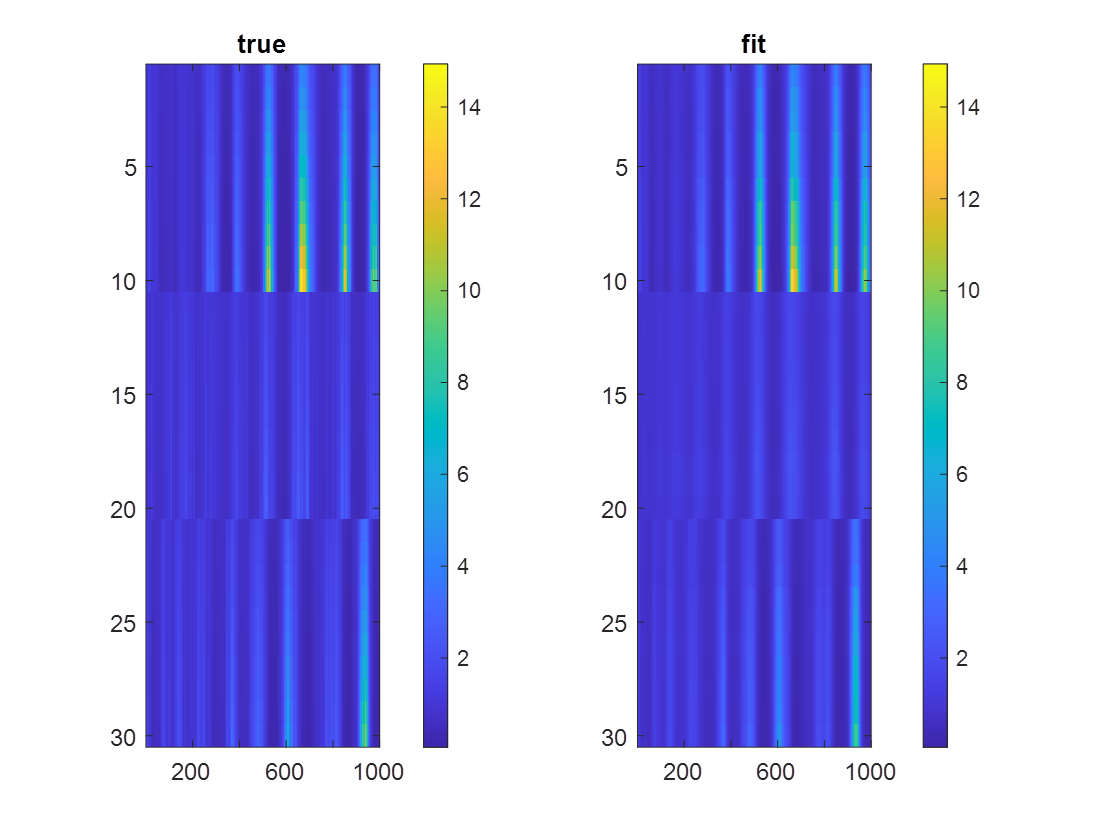
\includegraphics[width=0.55\textwidth]{image001.png}}%
		\subfigure[latents]{\label{fig:b}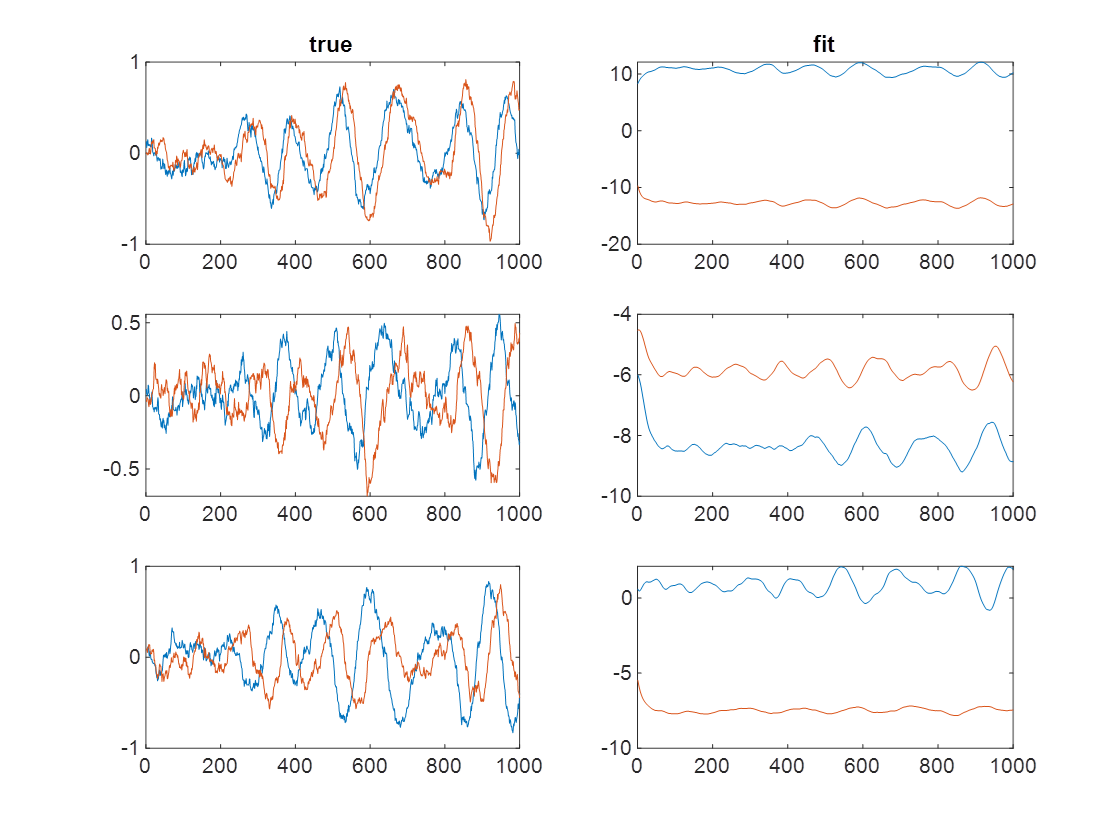
\includegraphics[width=0.55\textwidth]{image002.png}}%
		\subfigure[dynamics \(\mathbf{A}\)]{\label{fig:c}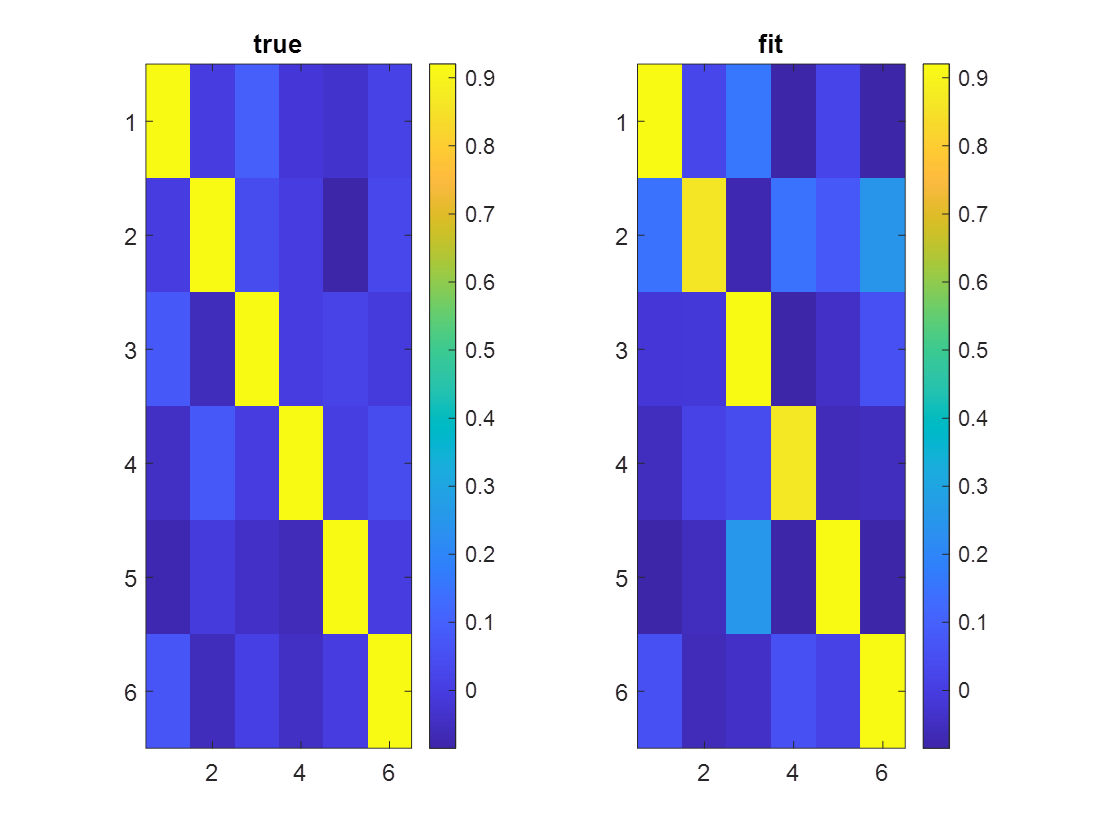
\includegraphics[width=0.55\textwidth]{image003.png}}%
	}
	\caption{LDS sample with labels}
	\label{fig:LDS labeled}
\end{figure}

The fitting for overall mean firing rate is perfect and the dynamics pattern is mostly recovered. The fitting of latents is OK (\textcolor{red}{\textbf{may not be accurate enough}}\\) up to scale. In other words, the model captures the oscillating pattern of latents.

But the latent patterns of these three clusters seems quite similar. That means the differences in the mean firing rates may be purely explained by the loading, i.e. \(\mathbf{d}\) and \(\mathbf{C}\). To see that, I set the number of cluster to be 1 and the results are shown in Figure \ref{fig:LDS labeled one cluster}.

\begin{figure}[h!]
	\makebox[\linewidth][c]{%
		\centering
		\subfigure[overall mean firing rate]{\label{fig:a}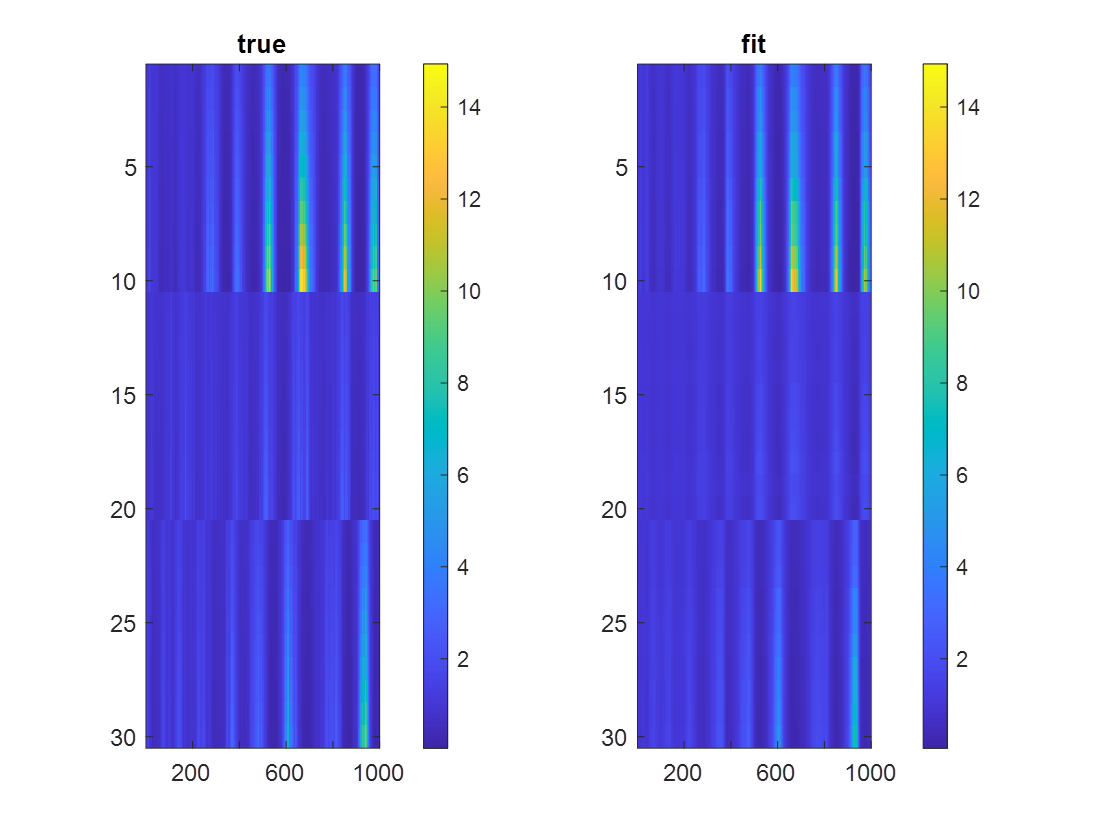
\includegraphics[width=0.7\textwidth]{image004.png}}%
		\subfigure[latents]{\label{fig:b}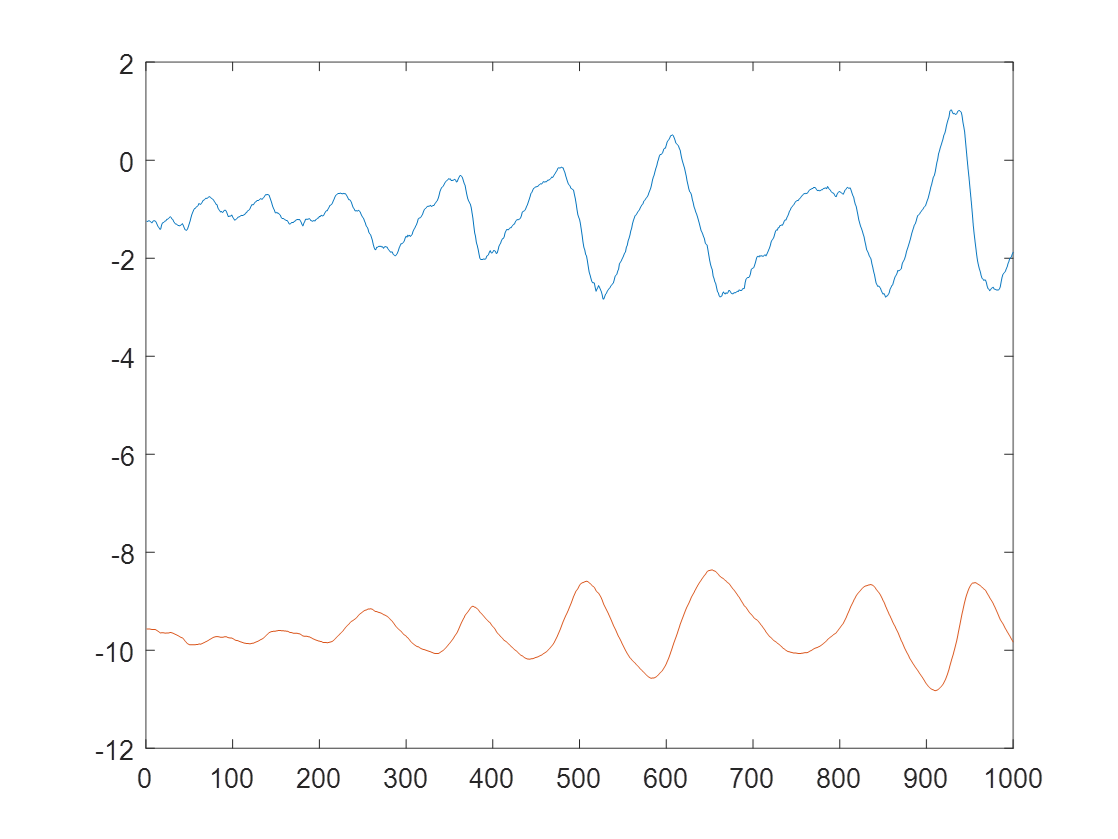
\includegraphics[width=0.7\textwidth]{image005.png}}%
	}
	\caption{LDS sample with labels, one cluster}
	\label{fig:LDS labeled one cluster}
\end{figure}

Again, the fitting for overall mean firing rate is perfect. This is why it's important to make the loading, \(\mathbf{d}\) and \(\mathbf{C}\), also be cluster-dependent (loading within clusters are correlated). If the loading only depends on neuron index and will not change for different clustering assignments, it's impossible to do clustering (at least in this case), since the loading is enough to capture all the patterns.

\subsubsection{Unlabeled Data: Clustering}
To give the full path of clustering, I show results in GIFs. Click to see the code for \href{https://github.com/weigcdsb/state-space-clustering/blob/main/LDS/lds_sample_MM.m}{FMM} and \href{https://github.com/weigcdsb/state-space-clustering/blob/main/LDS/lds_sample_DP.m}{DPMM}.

There are three results:
\begin{enumerate}
	\def\labelenumi{(\arabic{enumi})}
	\item
	Fit by FMM with \(J = 3\), starting from random cluster assignments:
	\href{https://github.com/weigcdsb/state-space-clustering/blob/main/results/gif/lds_samp_10_MM_above.gif}{GIF result 1}
	\item
	Fit by FMM with \(J = 3\), starting from all neurons in single cluster: 
	\href{https://github.com/weigcdsb/state-space-clustering/blob/main/results/gif/lds_samp_10_MM_below.gif}{GIF result 2}
	\item
	Fit by DPMM (\(\alpha = 10\)), starting from each neuron forms its own cluster:
	\href{https://github.com/weigcdsb/state-space-clustering/blob/main/results/gif/lds_samp_10_DP_above_10.gif}{GIF result 3}
	
\end{enumerate}
I didn't show the DPMM starting from single cluster. Since in my current implementation, the cluster generation is not efficient. In other words, the newly generated cluster will usually not be sampled and the algorithm usually gets stuck in 1 or 2 clusters.

This is a big problem... That means if we occasionally combine two clusters into one, we may never correct the mistake. Further, when the data grows, the number of cluster will be hard to grow. Fix that later.

\subsection{Simulation 2: Generate Latents, without Specifying Linear Dynamics}
In this simulation, there are again 3 clusters with 2 latents in each. Besides set 10 neurons in each cluster, I further simulate 50 neurons in each cluster to see performance in a larger scale. Now, the latents are generated directly without specifying the underlying linear dynamics of latents. However, each latent is generated independently, so the linear dynamics matrix \(\mathbf{A}\) should be roughly diagonal. The details of simulation can be found in the \href{https://github.com/weigcdsb/state-space-clustering/blob/main/LDS/unspecifiedA_sample.m}{code}.

\subsubsection{Labeled Data: No Clustering}
As in simulation 1, the data is fitted by the true cluster assignment (3 clusters) and forcing all neurons belong to single cluster. The code can be found \href{https://github.com/weigcdsb/state-space-clustering/blob/main/LDS/unspecifiedA_sample.m}{here}.
\begin{enumerate}
	\def\labelenumi{(\arabic{enumi})}
	\item
	Smaller dataset (10 neurons each):\\
	The results with true cluster assignment is shown in Figure \ref{fig:no A labeled 10}
	\begin{figure}[h!]
		\makebox[\linewidth][c]{%
			\centering
			\subfigure[overall mean firing rate]{\label{fig:a}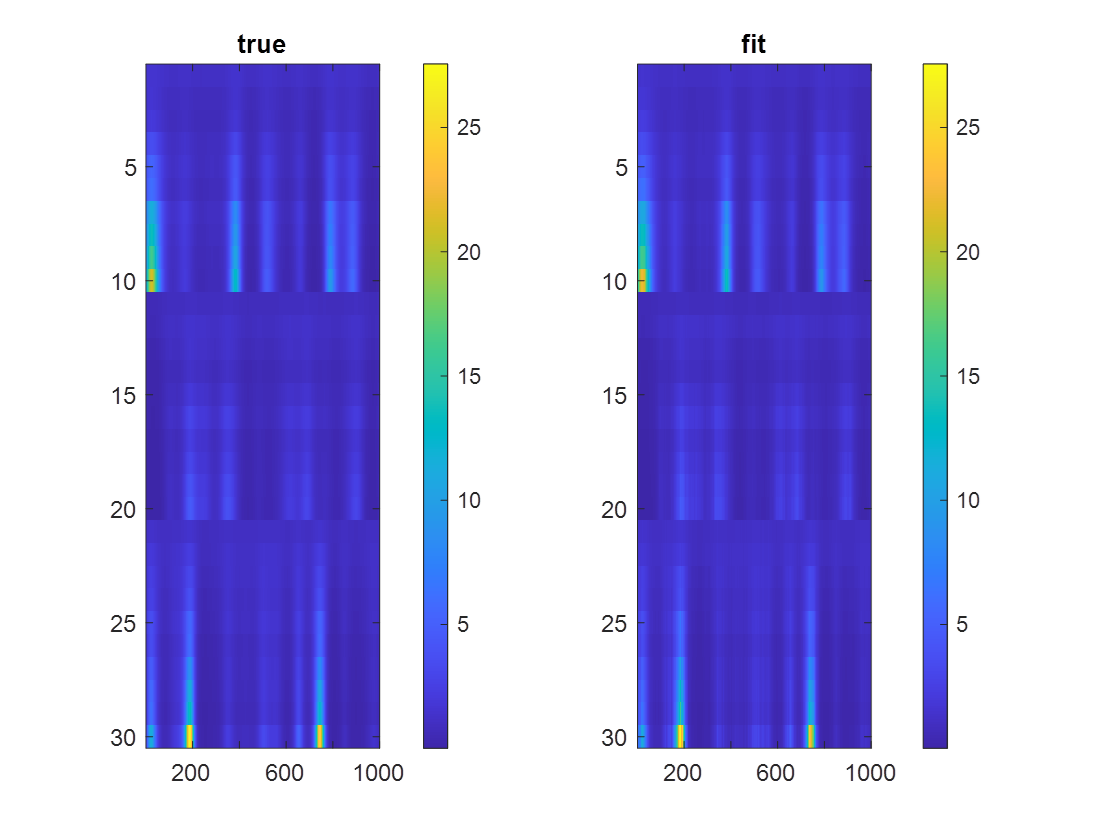
\includegraphics[width=0.55\textwidth]{image006.png}}%
			\subfigure[latents]{\label{fig:b}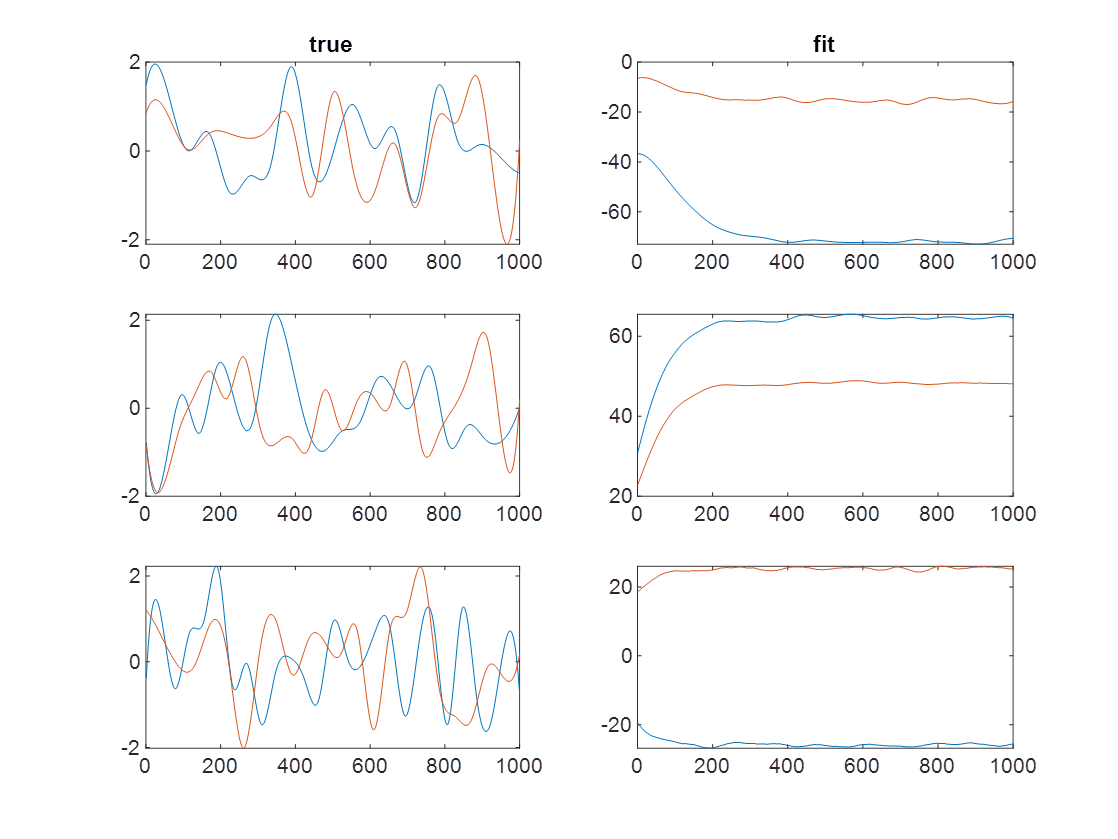
\includegraphics[width=0.55\textwidth]{image007.png}}%
			\subfigure[dynamics \(\mathbf{A}\)]{\label{fig:c}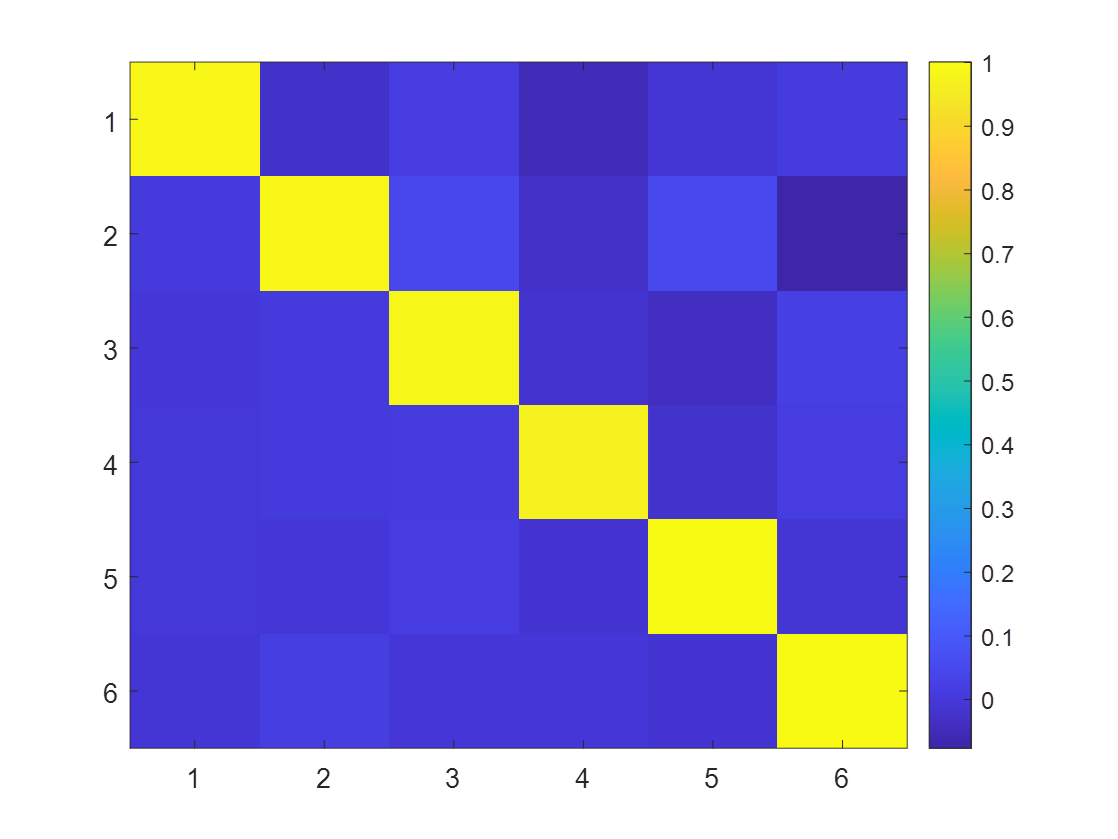
\includegraphics[width=0.55\textwidth]{image008.png}}%
		}
		\caption{unspecified dynamics with labels, 10 neurons each}
		\label{fig:no A labeled 10}
	\end{figure}
	And results by forcing all neurons to be in single cluster (Figure \ref{fig:no A labeled one cluster 10})
	\begin{figure}[h!]
		\makebox[\linewidth][c]{%
			\centering
			\subfigure[overall mean firing rate]{\label{fig:a}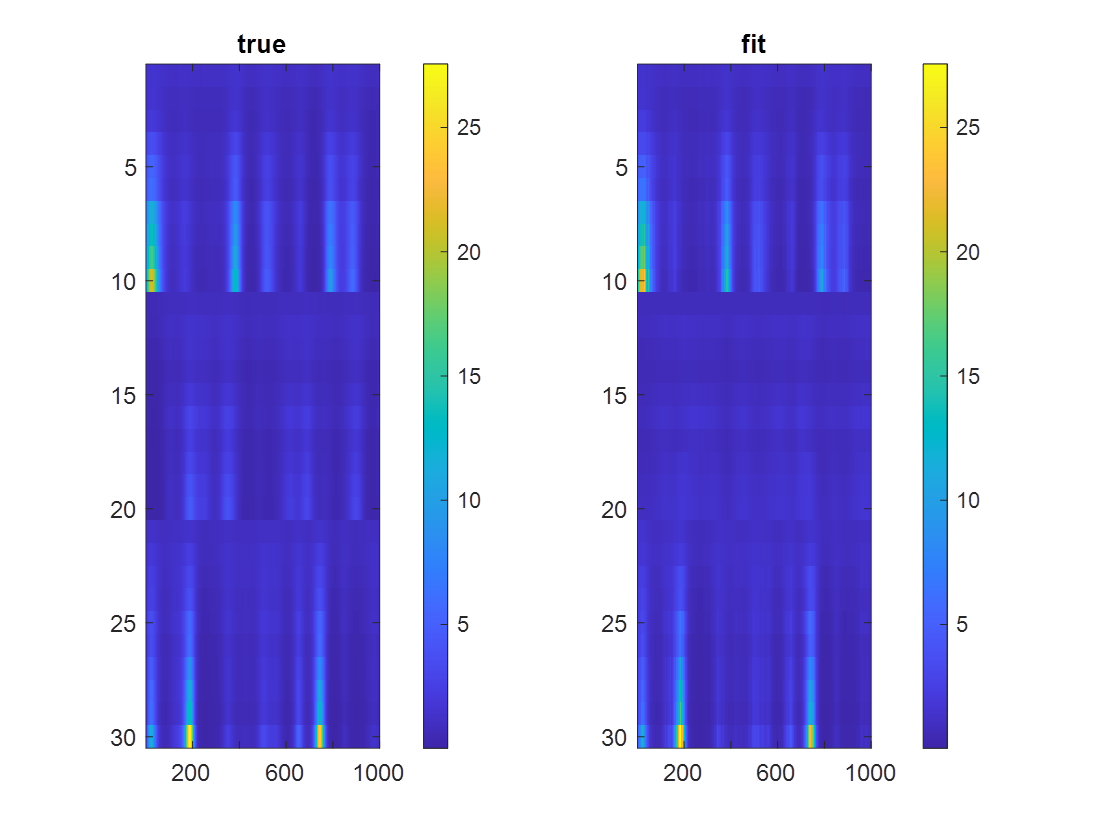
\includegraphics[width=0.7\textwidth]{image009.png}}%
			\subfigure[latents]{\label{fig:b}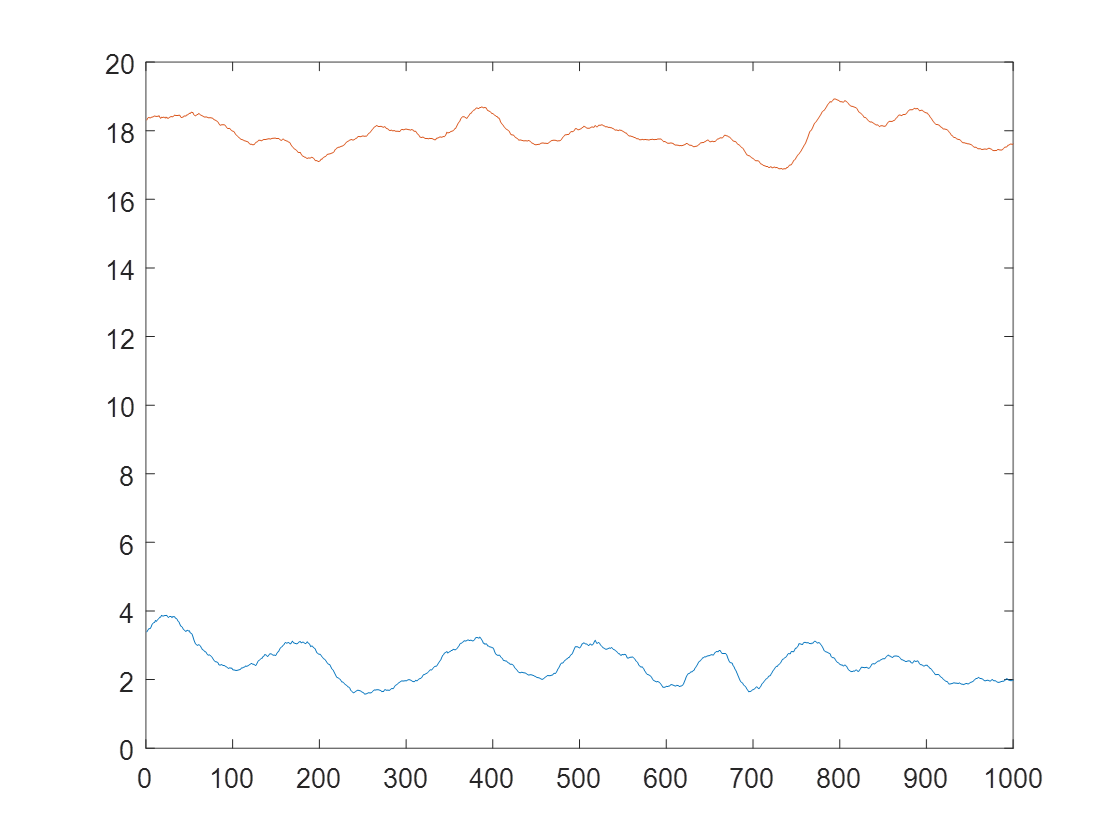
\includegraphics[width=0.7\textwidth]{image010.png}}%
		}
		\caption{unspecified dynamics with labels, one cluster, 10 neurons each}
		\label{fig:no A labeled one cluster 10}
	\end{figure}

	Again, the fittings for overall mean firing rate are perfect in both cases and the dynamics is roughly diagonal. The oscillating pattern of fitted latents with true cluster index is not significant, because of plot scaling. The pattern is easier to see in the second fitting.
	
	\item
	Larger dataset (50 neurons each):\\
	The results with true cluster assignment is shown in Figure \ref{fig:no A labeled 50}
	\begin{figure}[h!]
		\makebox[\linewidth][c]{%
			\centering
			\subfigure[overall mean firing rate]{\label{fig:a}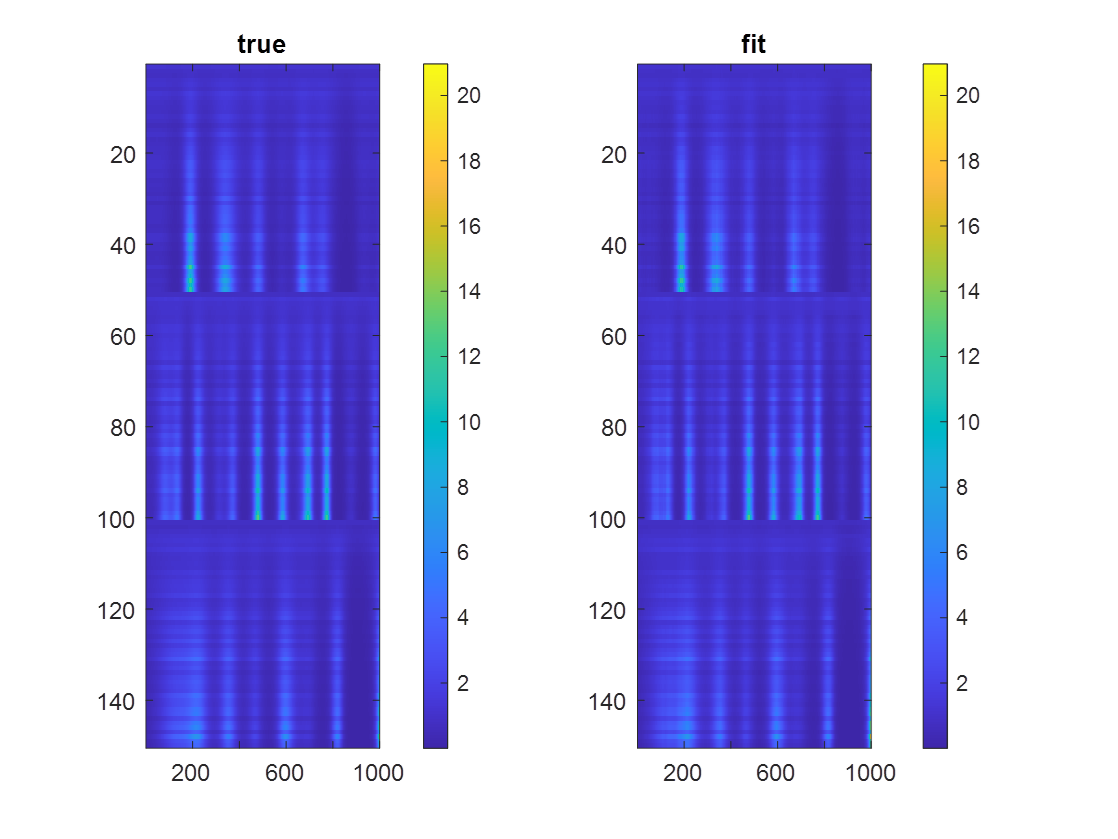
\includegraphics[width=0.55\textwidth]{image011.png}}%
			\subfigure[latents]{\label{fig:b}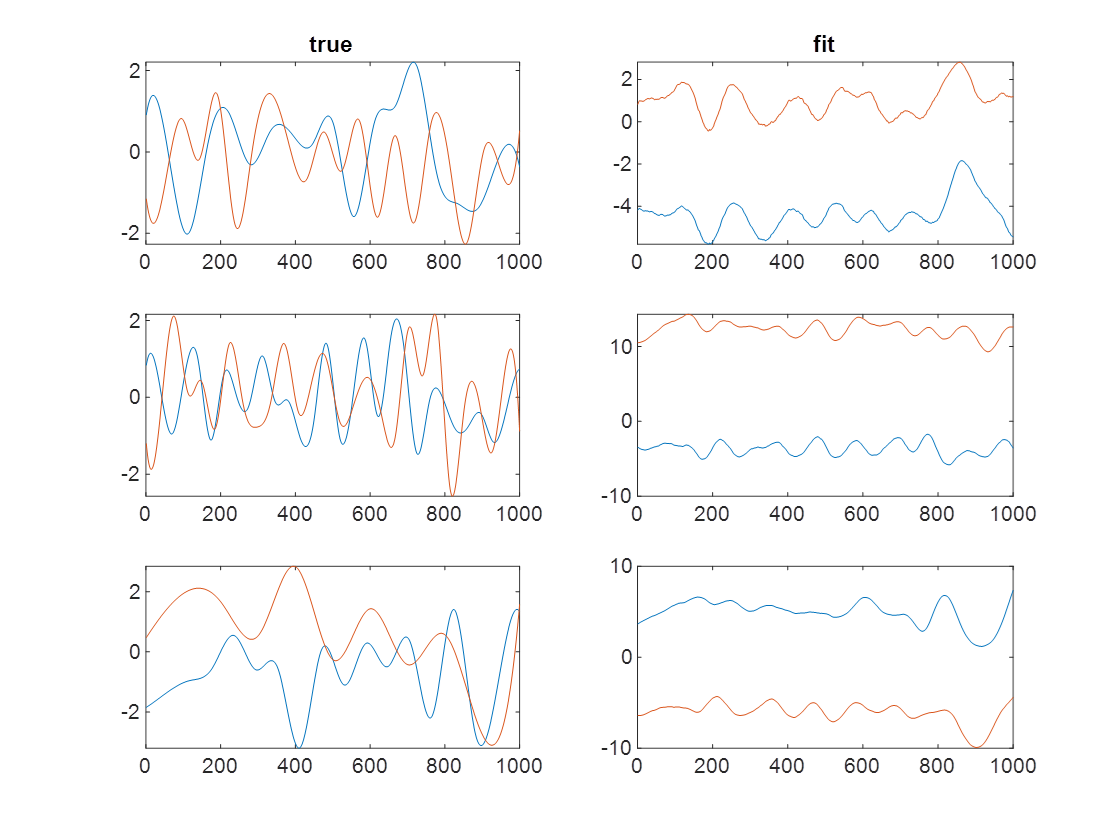
\includegraphics[width=0.55\textwidth]{image012.png}}%
			\subfigure[dynamics \(\mathbf{A}\)]{\label{fig:c}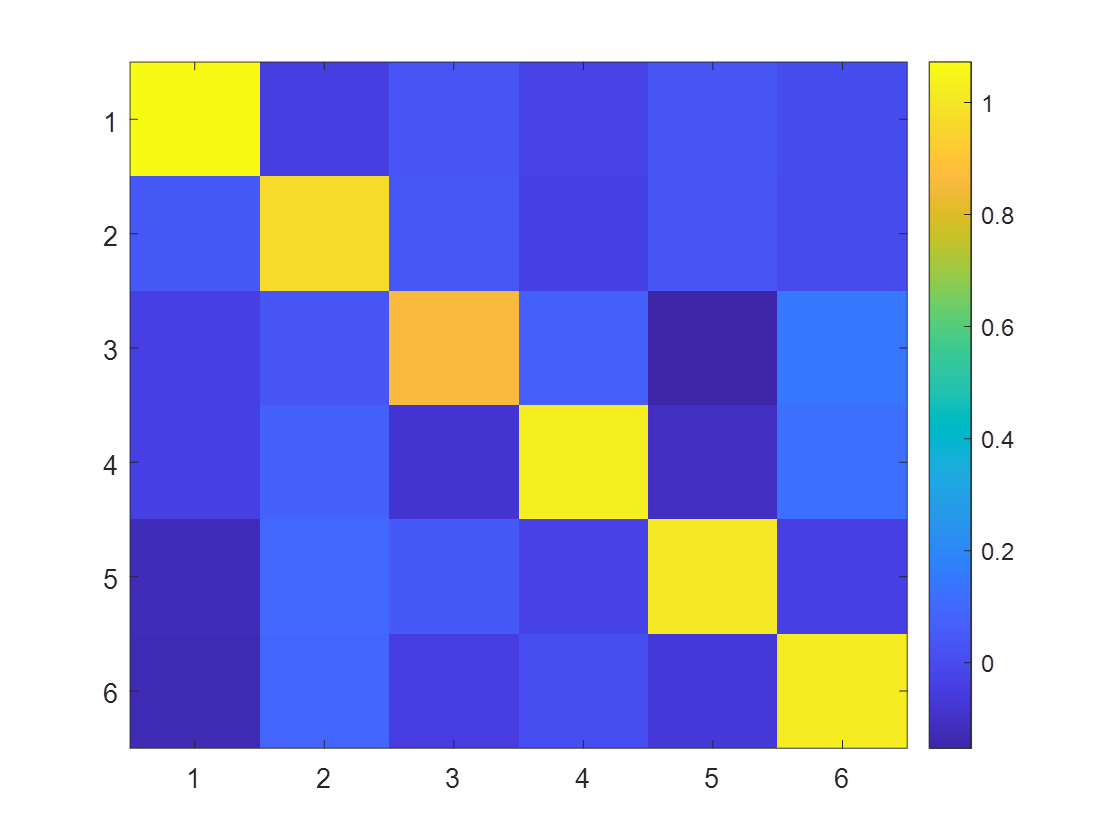
\includegraphics[width=0.55\textwidth]{image013.png}}%
		}
		\caption{unspecified dynamics with labels, 50 neurons each}
		\label{fig:no A labeled 50}
	\end{figure}
	And results by forcing all neurons to be in single cluster (Figure \ref{fig:no A labeled one cluster 50})
	\begin{figure}[h!]
		\makebox[\linewidth][c]{%
			\centering
			\subfigure[overall mean firing rate]{\label{fig:a}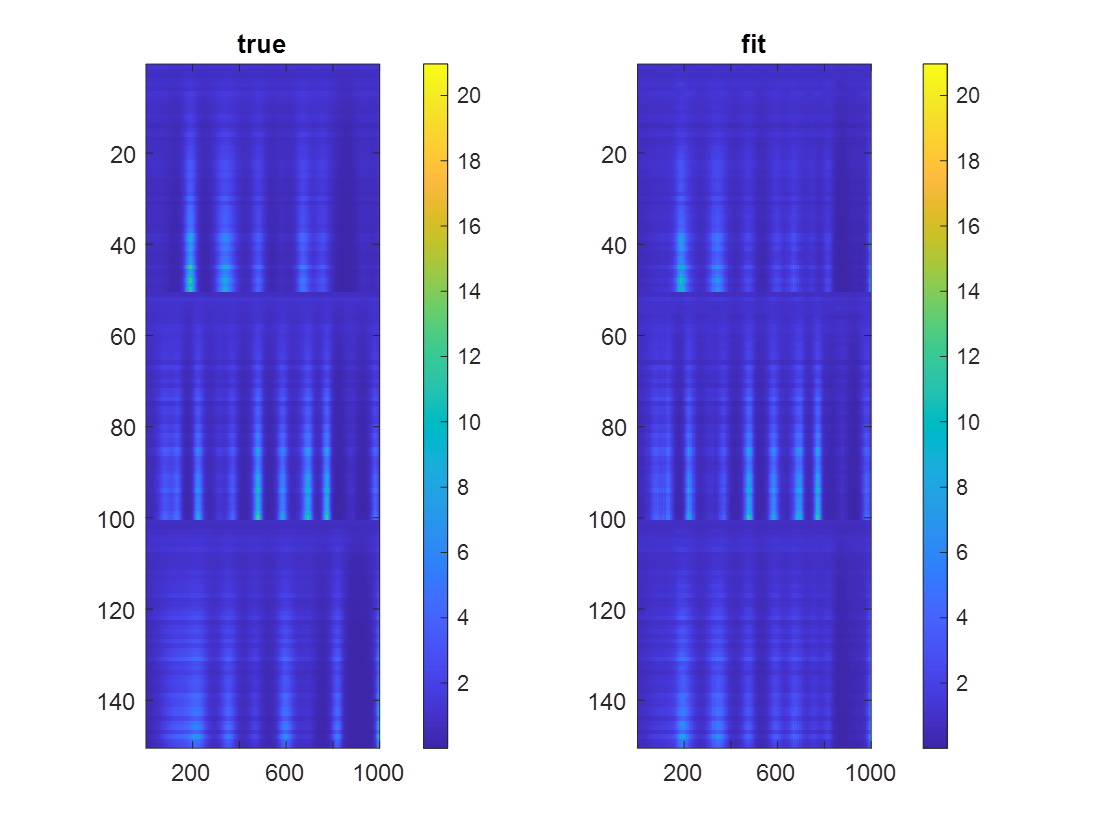
\includegraphics[width=0.7\textwidth]{image014.png}}%
			\subfigure[latents]{\label{fig:b}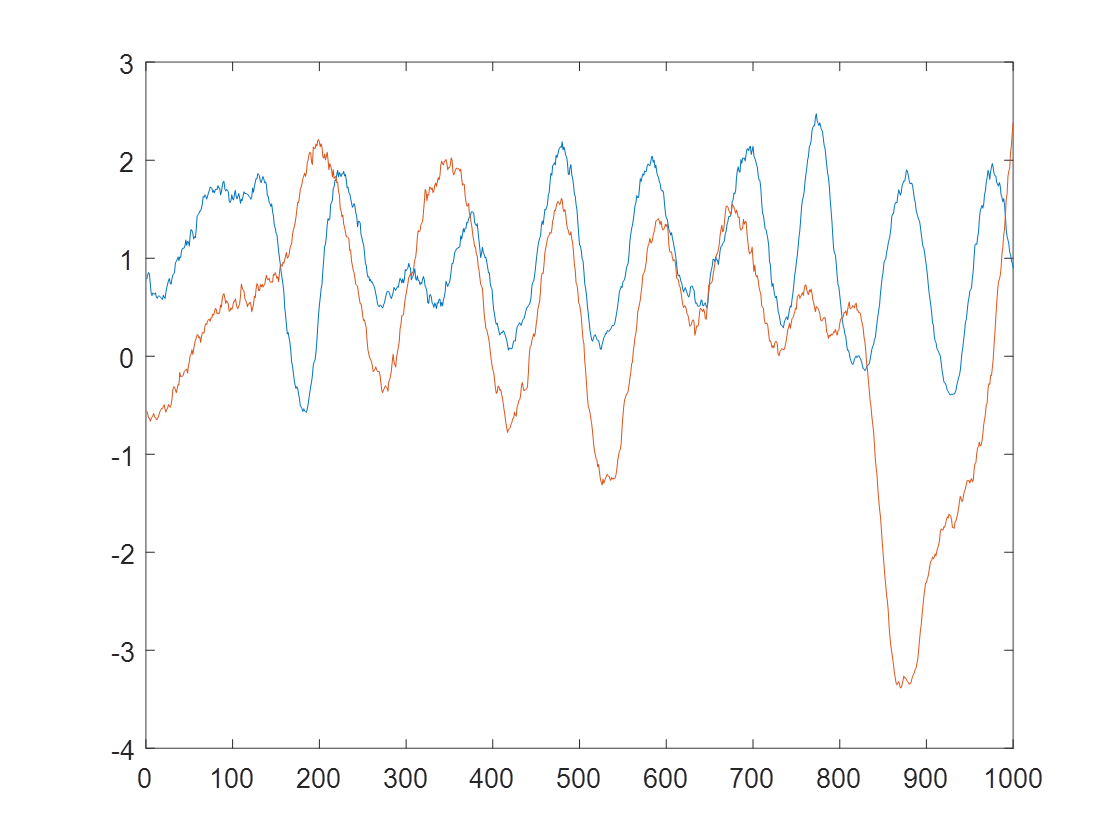
\includegraphics[width=0.7\textwidth]{image015.png}}%
		}
		\caption{unspecified dynamics with labels, one cluster, 50 neurons each}
		\label{fig:no A labeled one cluster 50}
	\end{figure}

	Now we can see the pattern more clearly.
\end{enumerate}

\subsubsection{Unlabeled Data: Clustering}
As previous, in each example, I show results from (1) FMM starting from random cluster assignment \(\left(J = 3\right) \), (2) FMM starting from single cluster and (3) DPMM starting from multiple clusters. The DPMM starting from single cluster need to be fixed later. These are code for
\href{https://github.com/weigcdsb/state-space-clustering/blob/main/LDS/unspecifiedA_sample_MM.m}{FMM} and \href{https://github.com/weigcdsb/state-space-clustering/blob/main/LDS/unspecifiedA_sample_DP.m}{DPMM}.

\begin{enumerate}
	\def\labelenumi{(\arabic{enumi})}
	\item
	Smaller dataset (10 neurons each):\\
	\begin{enumerate}
		\def\labelenumi{\alph{enumi}.}
		\item
		Fit by FMM with \(J = 3\), start from random cluster assignments:
		\href{https://github.com/weigcdsb/state-space-clustering/blob/main/results/gif/noA_10_MM_above.gif}{GIF result 4}
		\item
		Fit by FMM with \(J = 3\), start from single cluster:
		\href{https://github.com/weigcdsb/state-space-clustering/blob/main/results/gif/noA_10_MM_below.gif}{GIF result 5}
		\item
		Fit by DP (\(\alpha = 5\)), start from assuming each neuron forms its own cluster:
		\href{https://github.com/weigcdsb/state-space-clustering/blob/main/results/gif/noA_10_DP_above_5.gif}{GIF result 6}
	\end{enumerate}
	
	\item
	Larger dataset (50 neurons each):\\
	\begin{enumerate}
		\def\labelenumi{\alph{enumi}.}
		\item
		Fit by FMM with \(J = 3\), start from random cluster assignments:
		\href{https://github.com/weigcdsb/state-space-clustering/blob/main/results/gif/noA_50_MM_above.gif}{GIF result 7}
		\item
		Fit by FMM with \(J = 3\), start from single cluster:
		\href{https://github.com/weigcdsb/state-space-clustering/blob/main/results/gif/noA_50_MM_below.gif}{GIF result 8}
		\item
		Fit by DP (\(\alpha = 1\)), start from random assignment for 10 clusters:
		\href{https://github.com/weigcdsb/state-space-clustering/blob/main/results/gif/noA_50_DP_above1.gif}{GIF result 9}
	\end{enumerate}
\end{enumerate}

The performance is not bad. The neuron at top of each cluster cannot be clustered correctly by its nature: the signals are too weak to be clearly clustered.

\section{PROBLEMS} \label{problems}
This section shows what cause the inaccuracy in the latent estimation. 

\subsection{Estimation of \(\mathbf{d}\) and \(\mathbf{C}\) alone}
At first, as guessed by Ian, this may be caused by bad estimation of loading (\(\mathbf{d}\) and \(\mathbf{C}\)). So I first turn off all others except for loading (related) parameters and set them to be true values. There are 2 versions: (1) update priors as in subsection \ref{loading prior} and (2) no update of priors, and just set the prior for each as the standard normal.
For the estimation with prior update, the results are mean from iteration 50 to 100 (Figure \ref{loading alone}).
\begin{figure}[h!]
	\makebox[\linewidth][c]{%
		\centering
		\subfigure[]{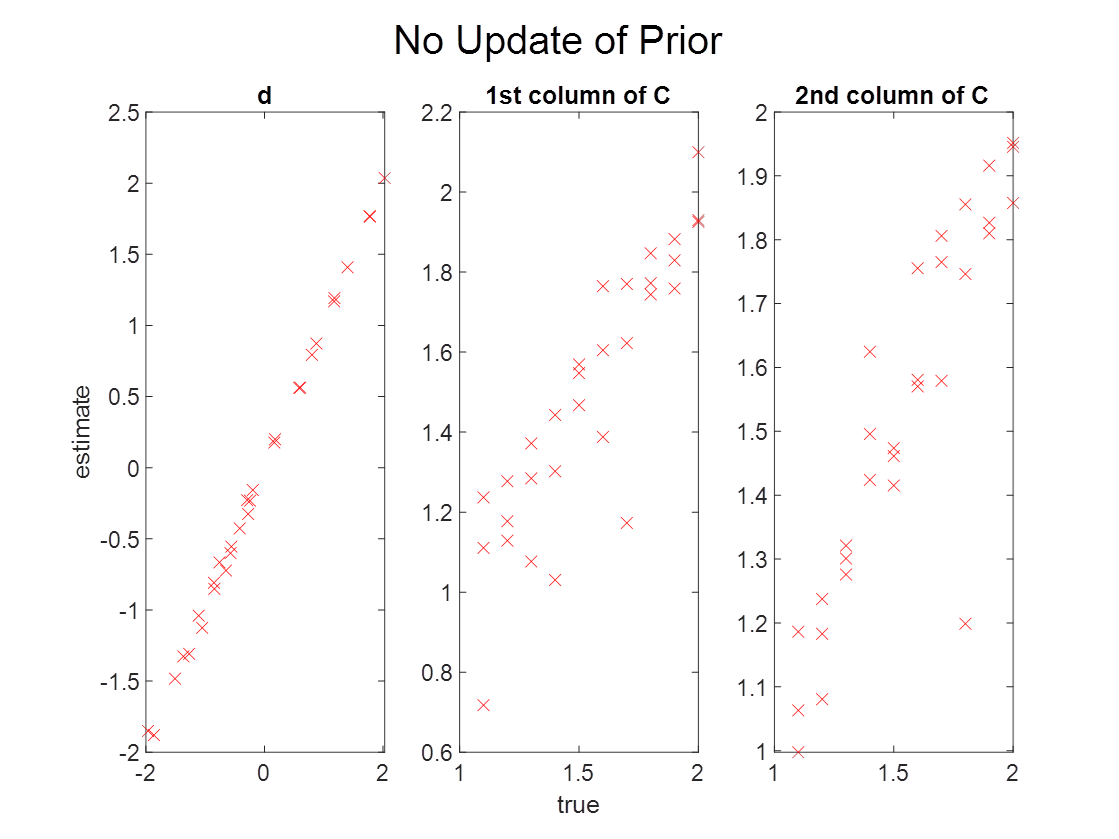
\includegraphics[width=0.6\textwidth]{image016.png}}%
		\subfigure[]{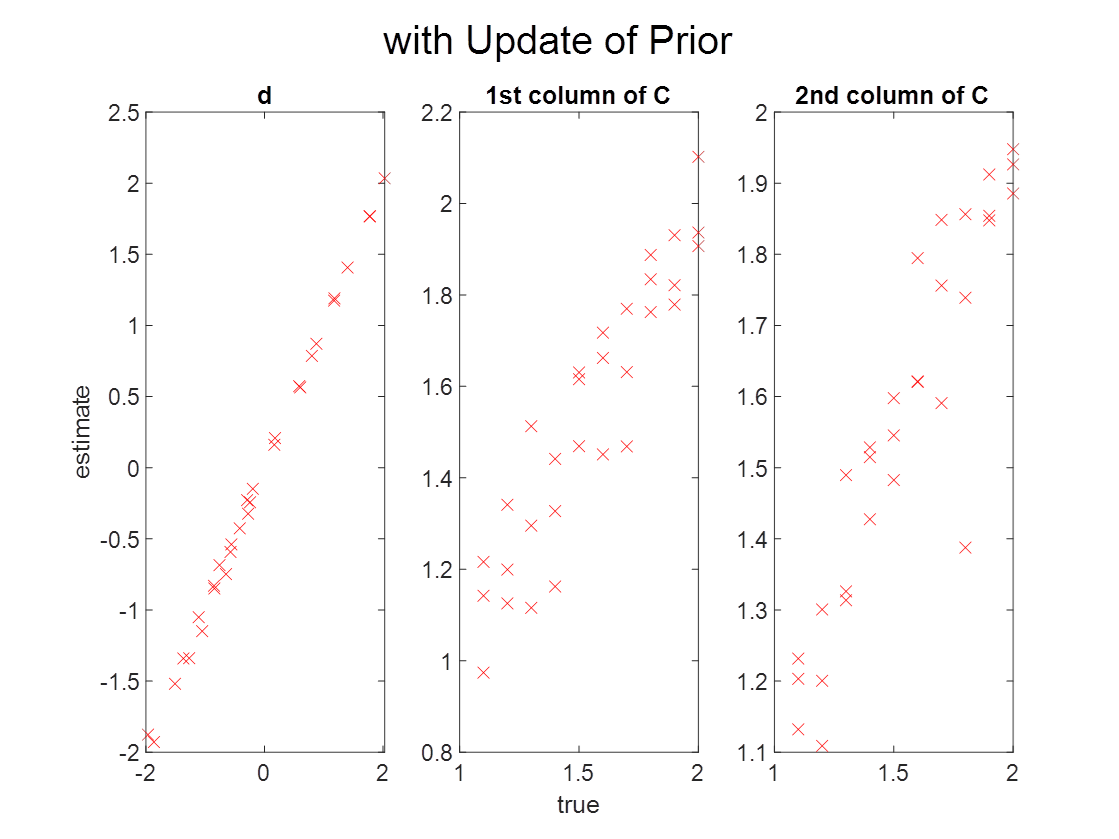
\includegraphics[width=0.6\textwidth]{image017.png}}%
	}
	\caption{estimation of loading}
	\label{loading alone}
\end{figure}
 
The mixing of convergence for loading priors (in subsection \ref{loading prior}) are fine. The update of priors don't influence results a lot, but this will help clustering a lot. It seems estimation of loading is fine. Let's see what happens when estimation of latents \(\mathbf{x}_t\) is on at the same time.

\subsection{Estimation of \(\mathbf{d}\), \(\mathbf{C}\) and \(\mathbf{x}_{t}\)}
When the estimation of \(\mathbf{x}_t\) is on, we need more iterations. The results are mean from iteration 500 to 1000 (Figure \ref{loading and latent}).

The estimation of loading:
\begin{figure}[h!]
	\makebox[\linewidth][c]{%
		\centering
		\subfigure[]{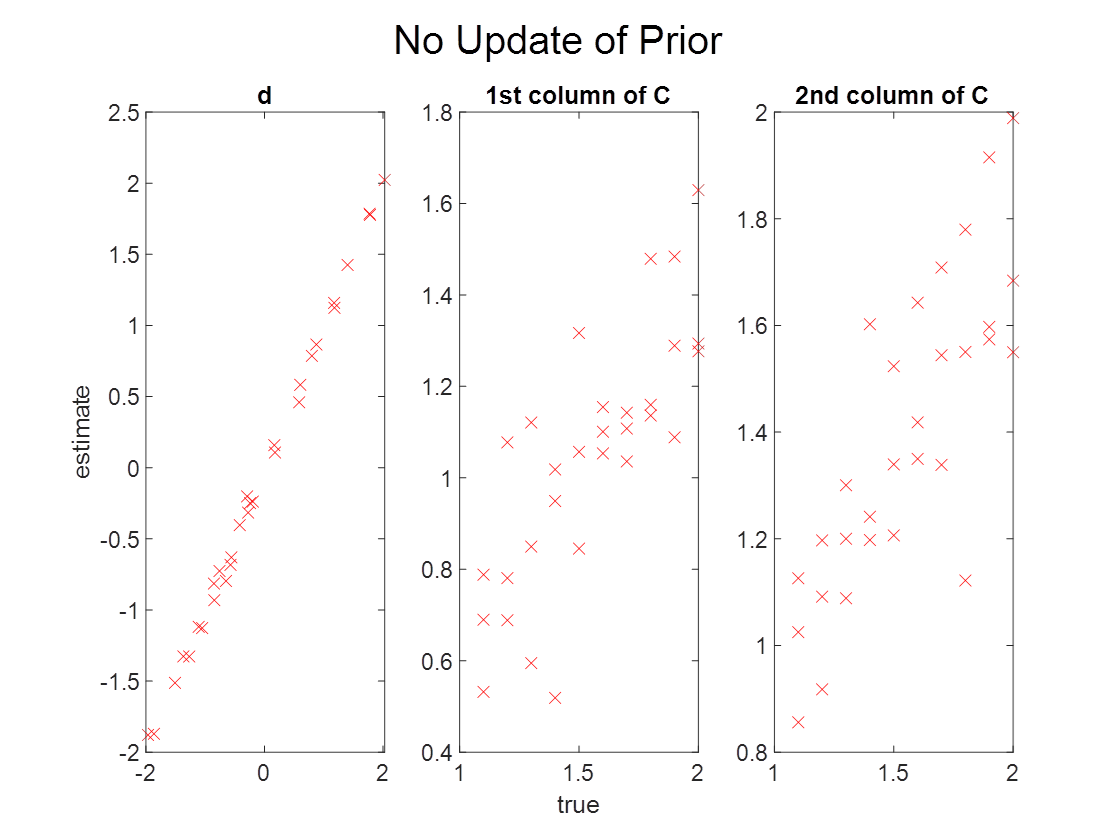
\includegraphics[width=0.6\textwidth]{image018.png}}%
		\subfigure[]{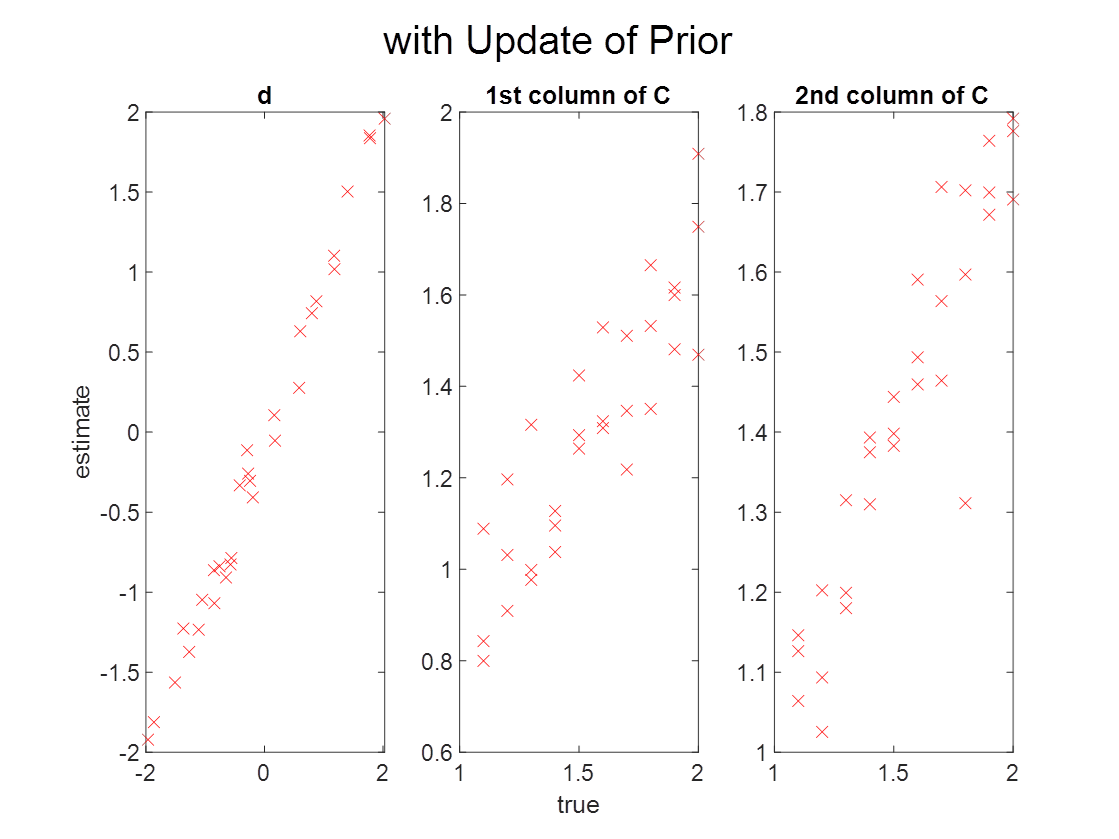
\includegraphics[width=0.6\textwidth]{image020.png}}%
	}
	\caption{estimation of loading, with latents on}
	\label{loading and latent}
\end{figure}

And the estimation of corresponding latents (Figure \ref{loading and latents}):
\begin{figure}[h!]
	\makebox[\linewidth][c]{%
		\centering
		\subfigure[no update of prior]{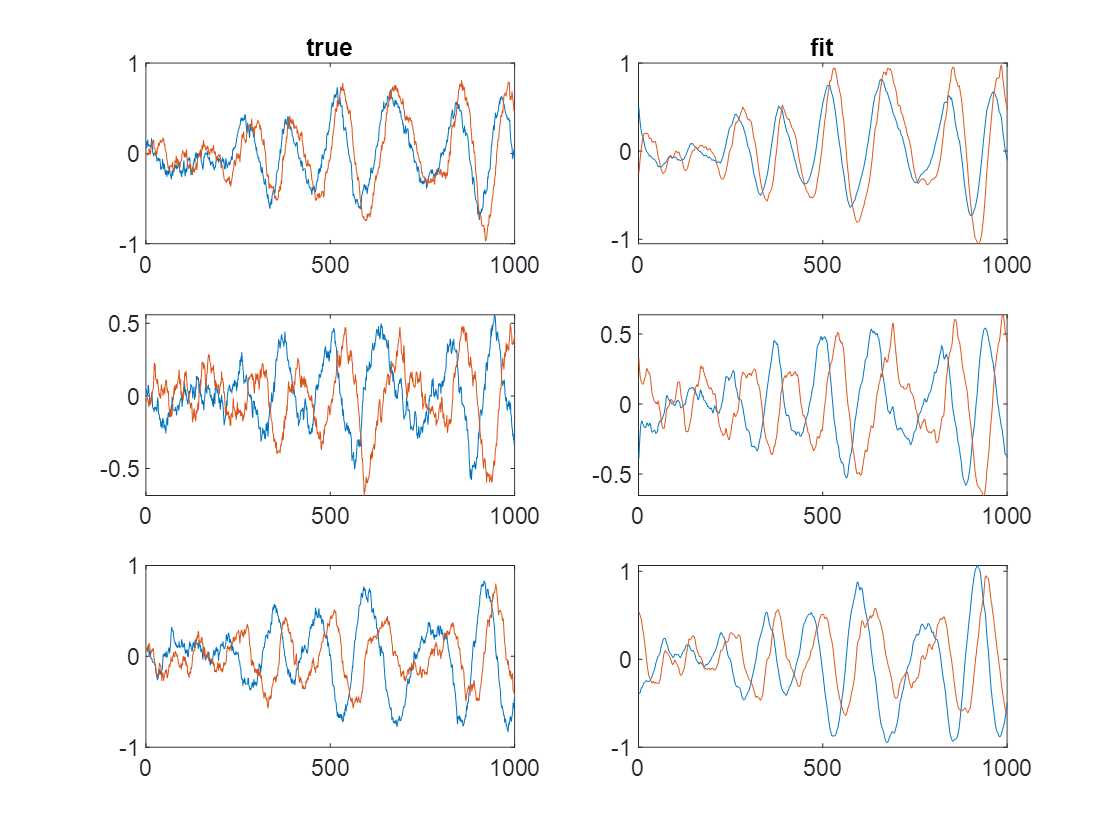
\includegraphics[width=0.6\textwidth]{image019.png}}%
		\subfigure[with update of prior]{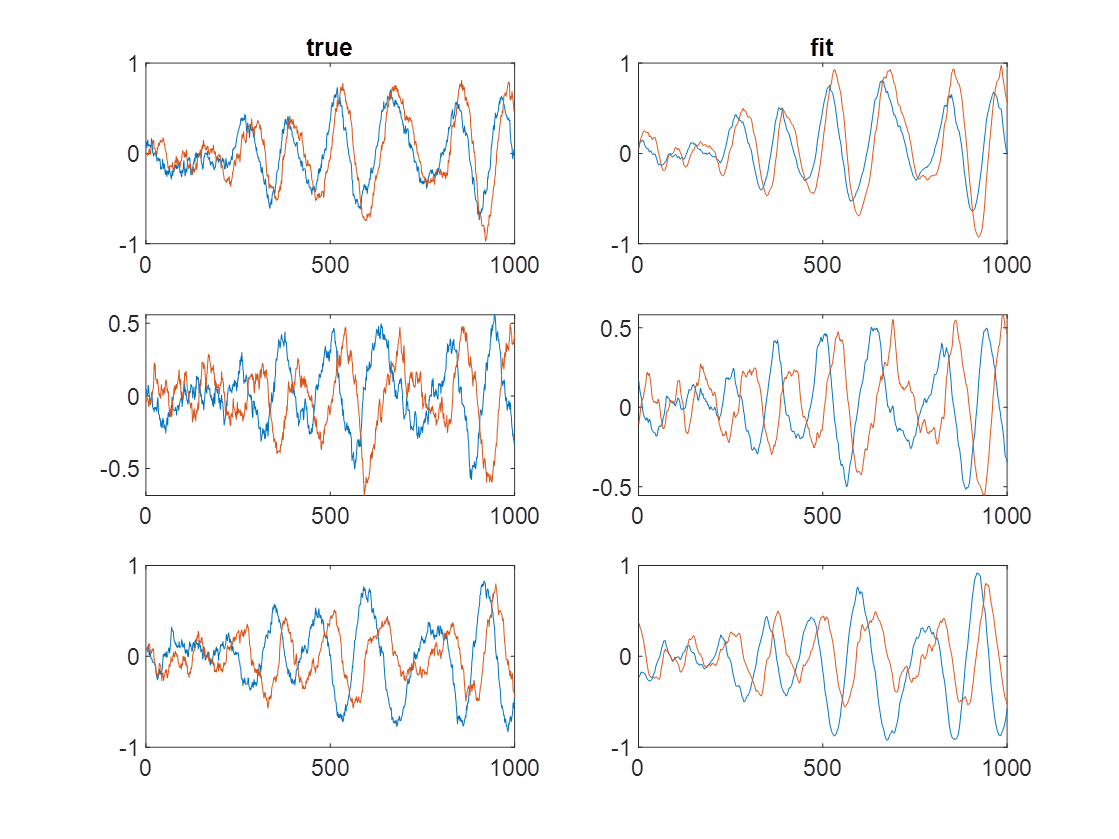
\includegraphics[width=0.6\textwidth]{image021.png}}%
	}
	\caption{estimation of loading}
	\label{loading and latents}
\end{figure}

Things are still fine. The remaining parts may influence latent estimations are dynamics (\(\mathbf{b}\), \(\mathbf{A}\)) and prior process noise \(\mathbf{Q}\).

I've checked update of (1) dynamics alone, (2) \(\mathbf{Q}\) and (3) \(\mathbf{Q}\) and \(\mathbf{x}_{t}\). All of them are fine. \textbf{So the problem must come from estimations of dynamics and \(\mathbf{x}_t\)}.

\subsection{Estimation of \(\mathbf{b}\), \(\mathbf{A}\) and \(\mathbf{x}_t\)}
I first estimate dynamics by assuming block diagonal \(\mathbf{Q}\) (as in subsection \ref{dynamics update}). When turning on (1) latents \(\mathbf{x}_t\) and (2) dynamics (\(\mathbf{b}\) and \(\mathbf{A}\)), the trace of \(\mathbf{b}\) and \(\mathbf{A}\) are (Figure \ref{trace of dynamics, blk}):\\
\begin{figure}[h!]
	\centering
	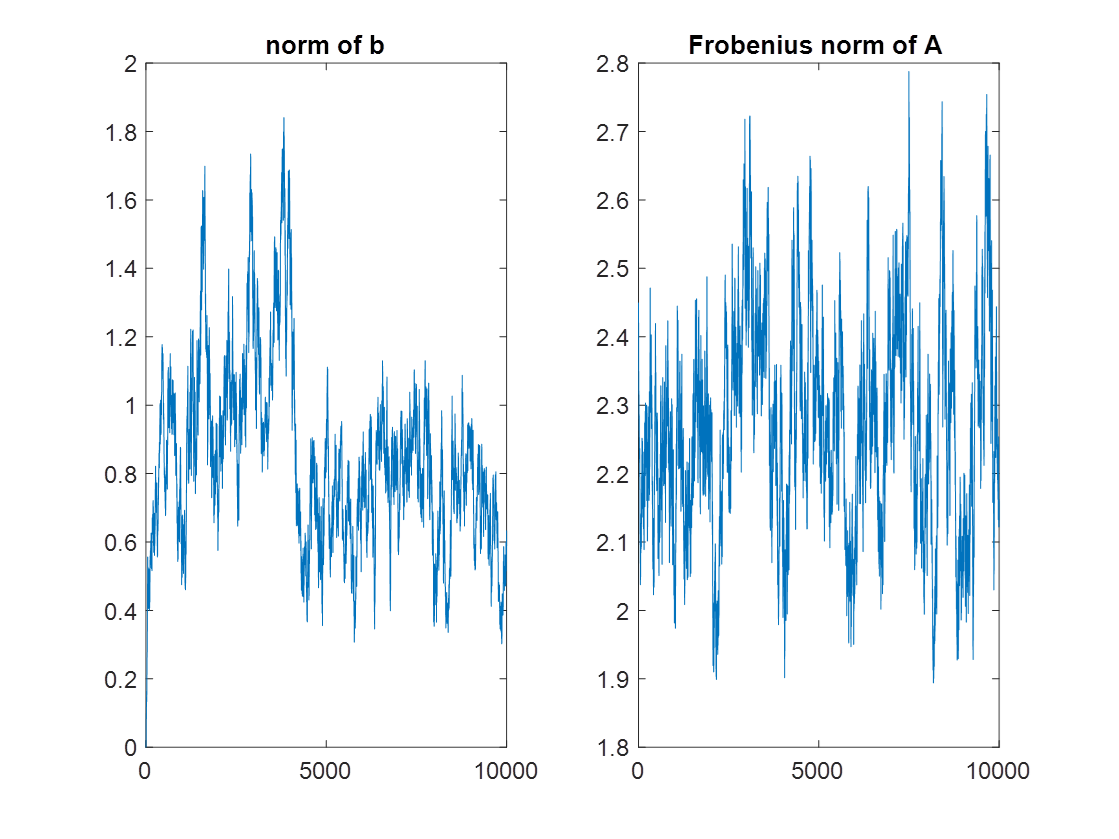
\includegraphics[width = .7\textwidth]{image022.png}
	\caption{trace of dynamics, block diagonal}
	\label{trace of dynamics, blk}
\end{figure}

The mixing is not good, and we may haven't achieve stationary distribution yet. Anyway, I average results from iteration 5000 to 10000, and the results are shown in Figure \ref{lat and dyn, blk}).
\begin{figure}[h!]
	\makebox[\linewidth][c]{%
		\centering
		\subfigure[latent]{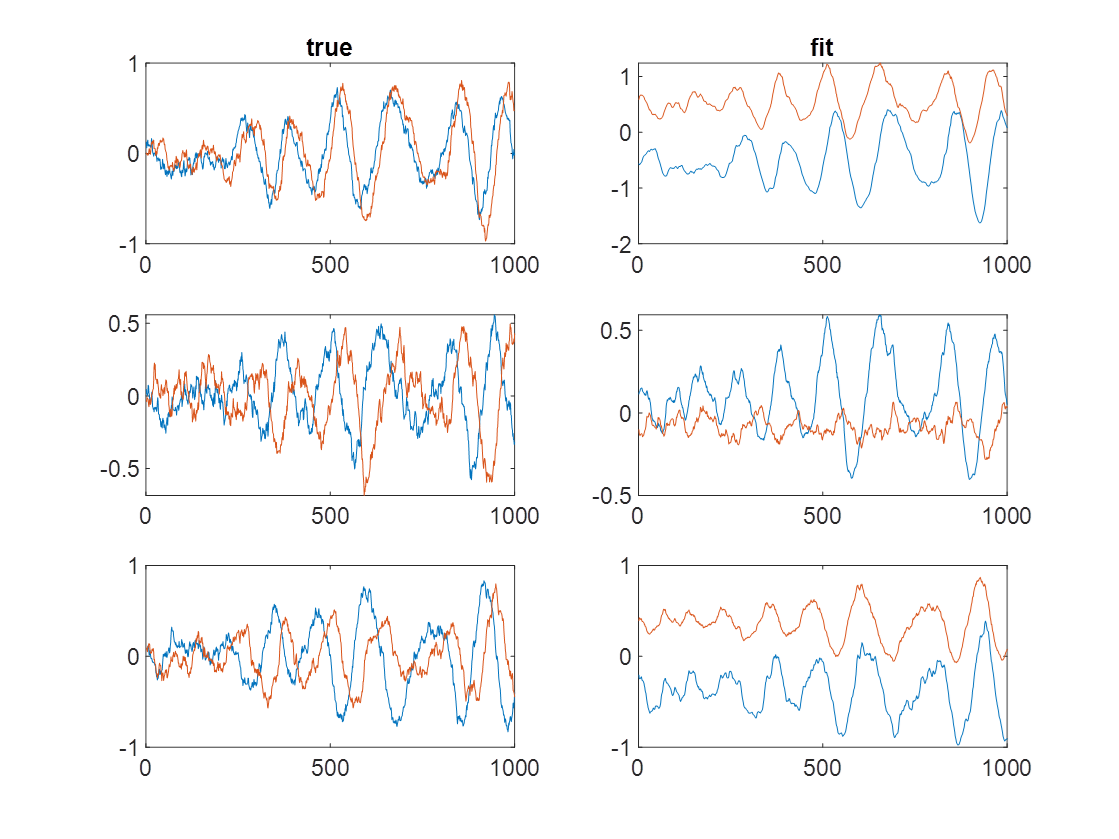
\includegraphics[width=0.6\textwidth]{image023.png}}%
		\subfigure[dynamics]{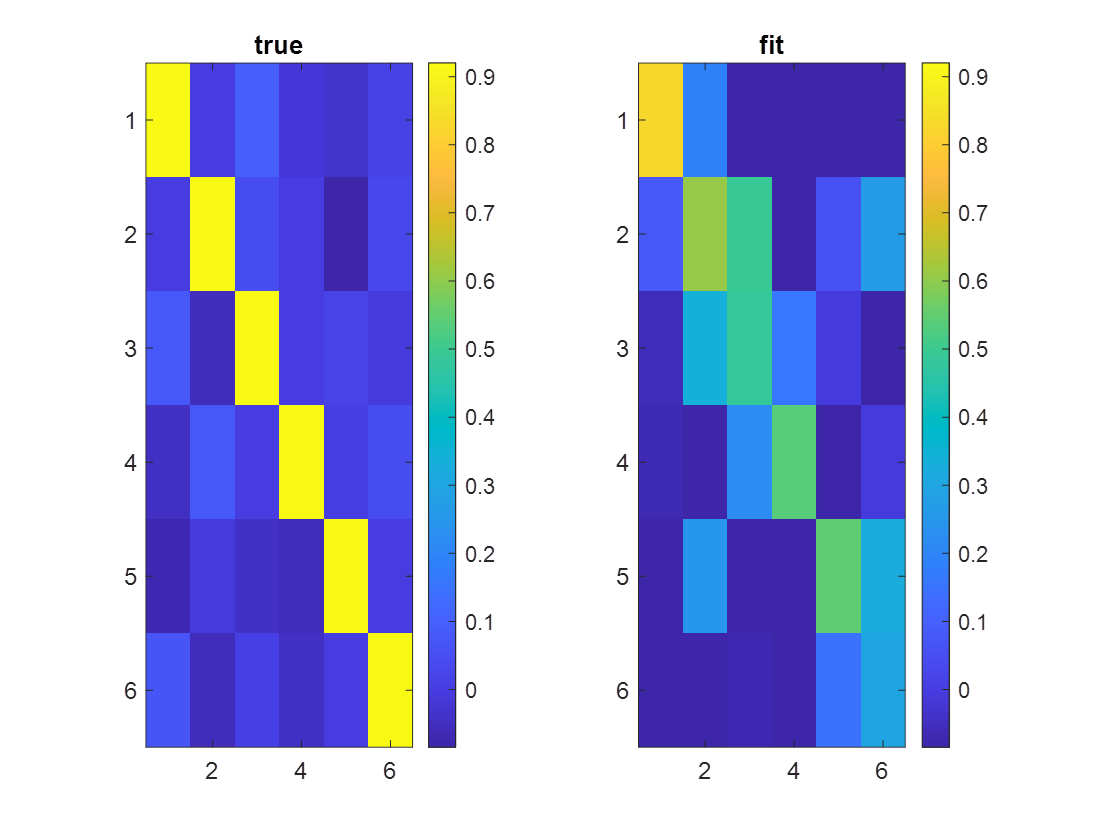
\includegraphics[width=0.6\textwidth]{image024.png}}%
	}
	\caption{estimation of latents and dynamics, block diagonal}
	\label{lat and dyn, blk}
\end{figure}

OK, things are not perfect now. What if I don't assume block diagonal \(\mathbf{Q}\)? For the non-constraint version, the trace plot of \(\mathbf{b}\) and \(\mathbf{A}\) are in Figure \ref{trace of dynamics, full}.
\begin{figure}[h!]
	\centering
	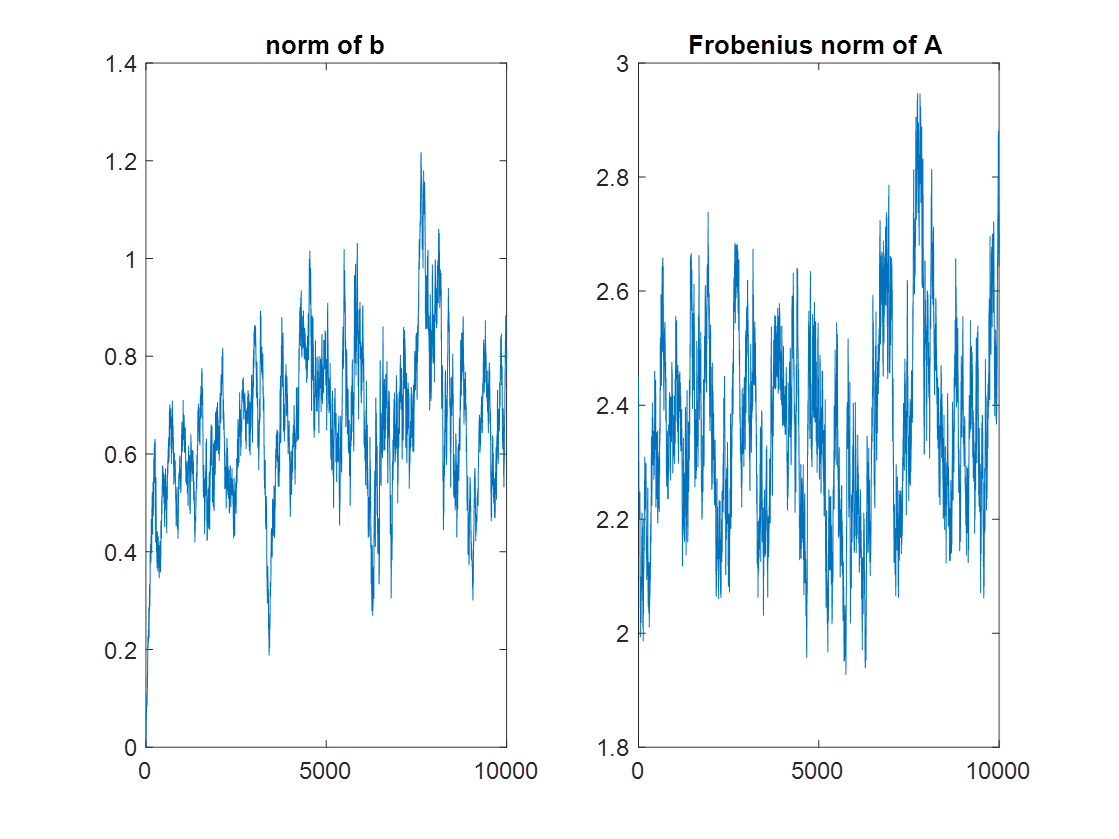
\includegraphics[width = .7\textwidth]{image025.png}
	\caption{trace of dynamics, no constraint}
	\label{trace of dynamics, full}
\end{figure}\\


Again, the average from iteration 5000 to 10000 is in Figure \ref{lat and dyn, full}).\\
\begin{figure}[h!]
	\makebox[\linewidth][c]{%
		\centering
		\subfigure[latent]{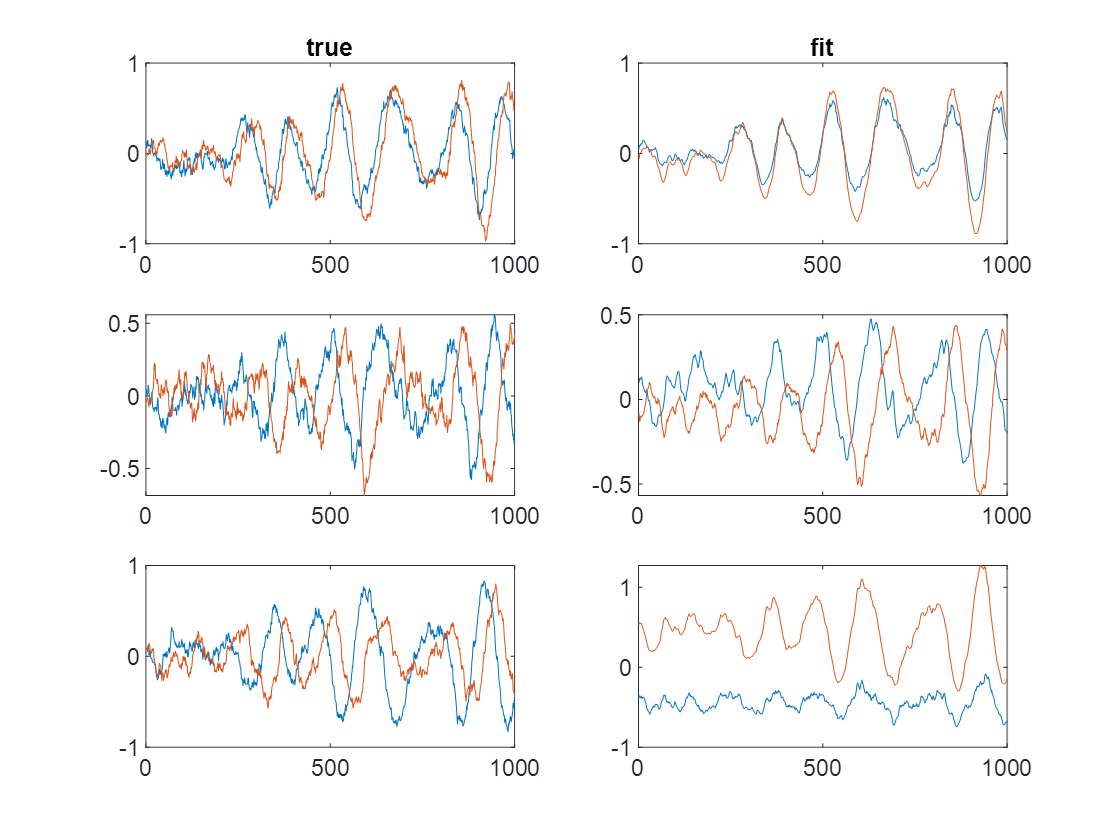
\includegraphics[width=0.6\textwidth]{image026.png}}%
		\subfigure[dynamics]{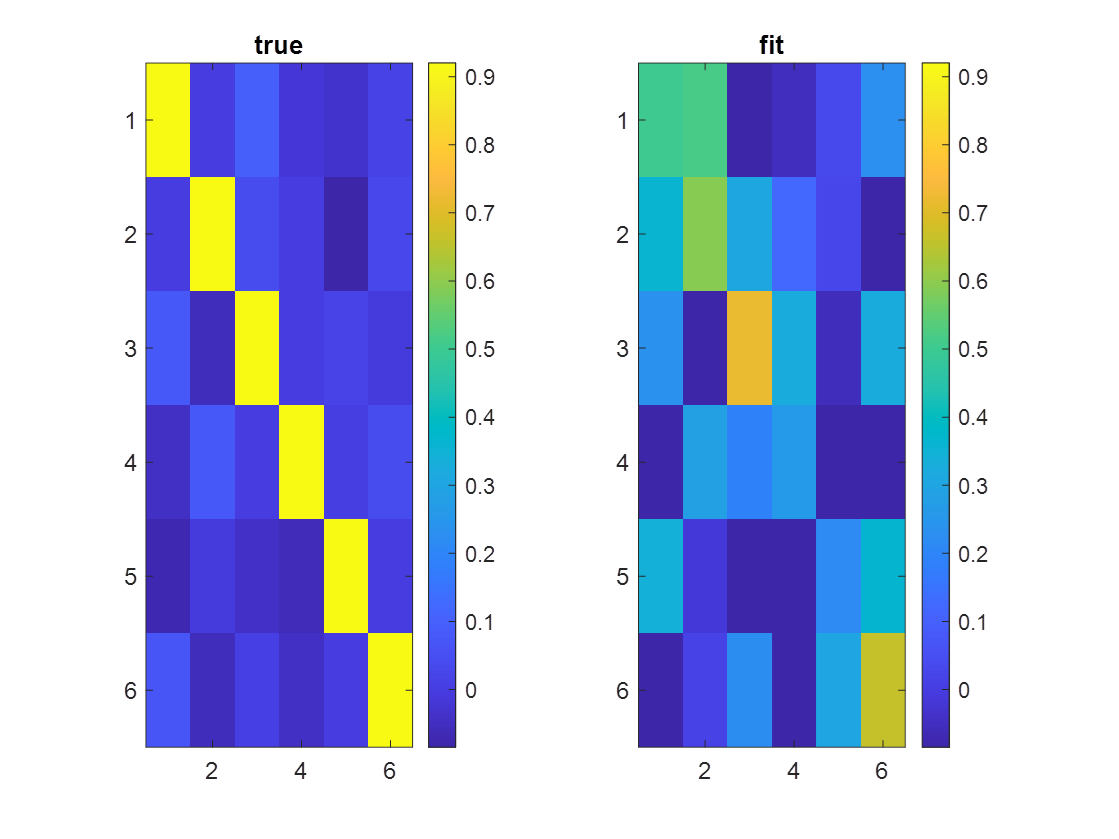
\includegraphics[width=0.6\textwidth]{image027.png}}%
	}
	\caption{estimation of latents and dynamics, no constraint}
	\label{lat and dyn, full}
\end{figure}

Based on trace plot and latent, things look a bit better. But it's still not good enough. The dynamics is even worse, although the latent is better.

\textbf{Another Observation}:
Even with these inaccurate latent, the overall mean firing rate still looks perfect (with true loading \(\mathbf{d}\) and \(\mathbf{C}\)), because of small loading. See Figure \ref{mfr, blk and full}

\begin{figure}[h!]
	\makebox[\linewidth][c]{%
		\centering
		\subfigure[block diagonal]{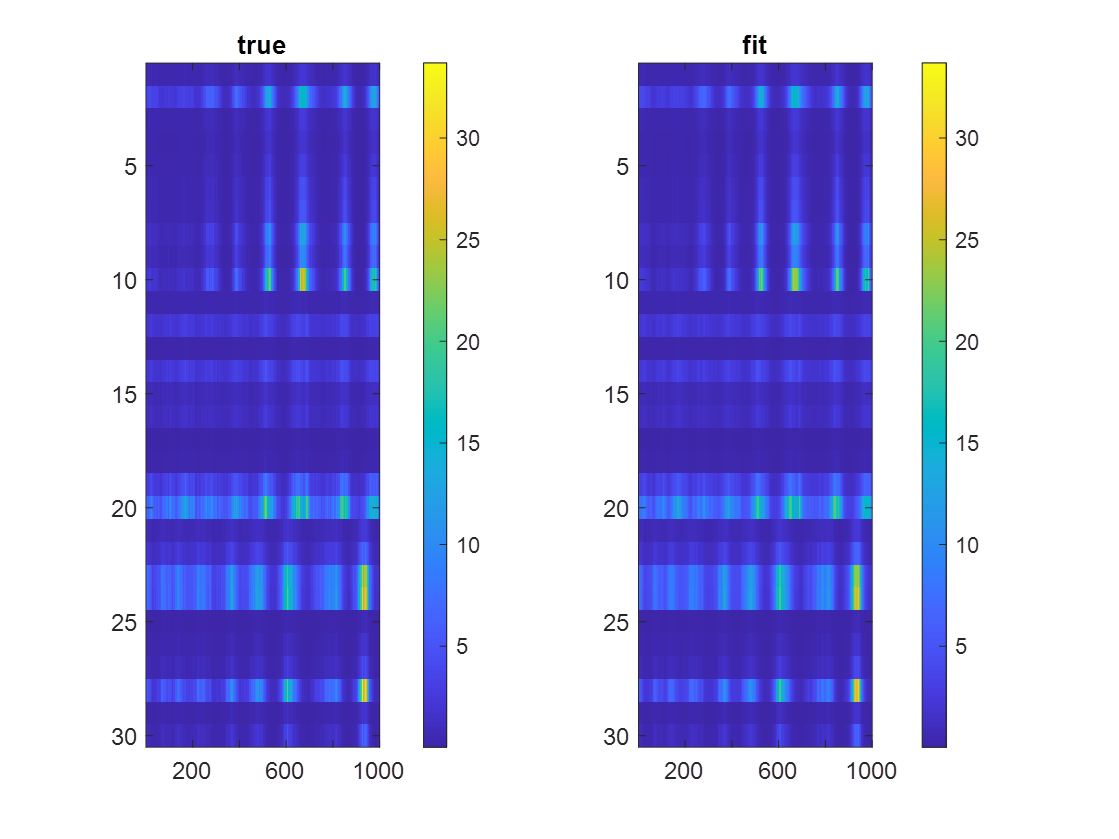
\includegraphics[width=0.6\textwidth]{image028.png}}%
		\subfigure[no constraint]{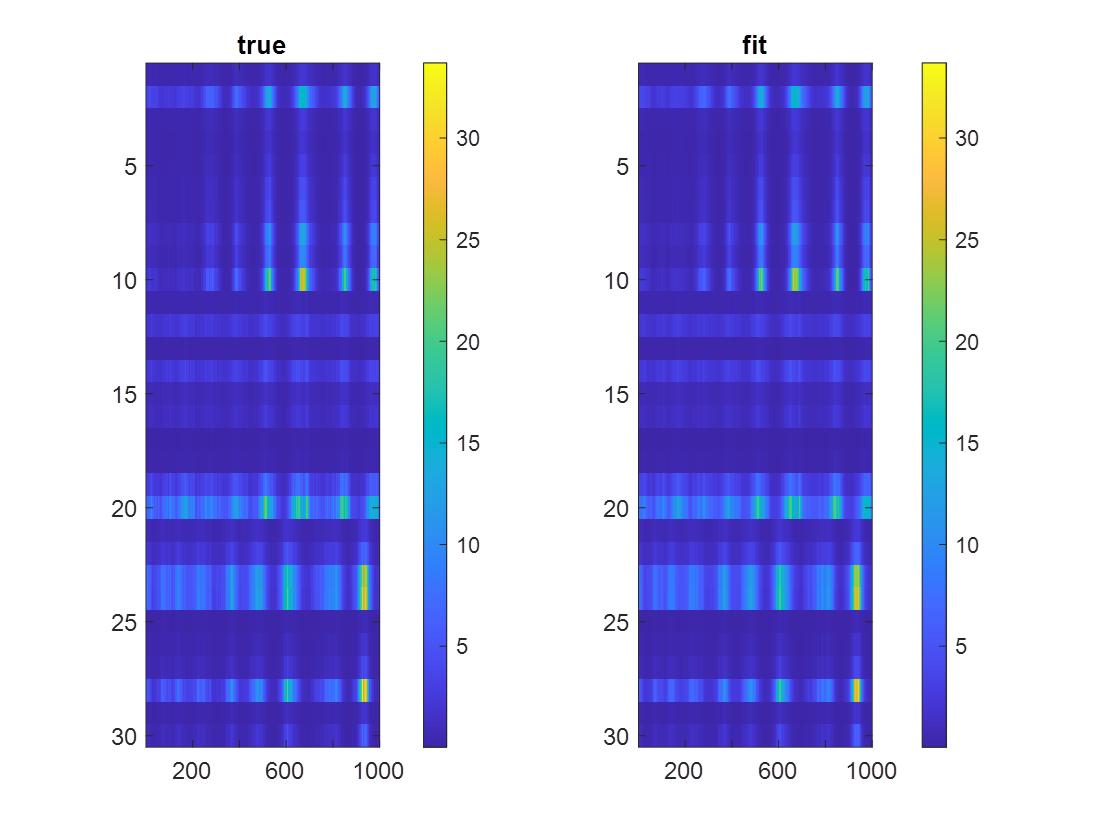
\includegraphics[width=0.6\textwidth]{image029.png}}%
	}
	\caption{overall mean firing rate, block diagonal and no constraint}
	\label{mfr, blk and full}
\end{figure}

In PLDS, they use EM, so there's no noise. But here I tackle things by MCMC: if the simulation is not very identifiable, then there will be a lot of noise by its nature.

Anyway, the clustering is based on the overall mean firing rate pattern. Although the estimation of latent may not be accurate enough, this should not influence the clustering result.

Maybe the next step is to test the current algorithm by a more identifiable simulation. For example, use a larger loading to make the latent effect become more significant.

\subsection{Simulation 1 Revisit}
The results above remind me that the 100 iterations is not enough to achieve stationary distribution. I need to check the sampling trace.
Here, I rerun the MCMC for simulation 1, but use the no-constraint \(\mathbf{Q}\) version. Since no constraint version is better than block-diagonal one.

First, I show the trace of sampling (Frobenius) norm for \(\mathbf{d}\), \(\mathbf{C}\), \(\mathbf{b}\) and \(\mathbf{A}\) as in Figure \ref{norms}.
\begin{figure}[h!]
	\centering
	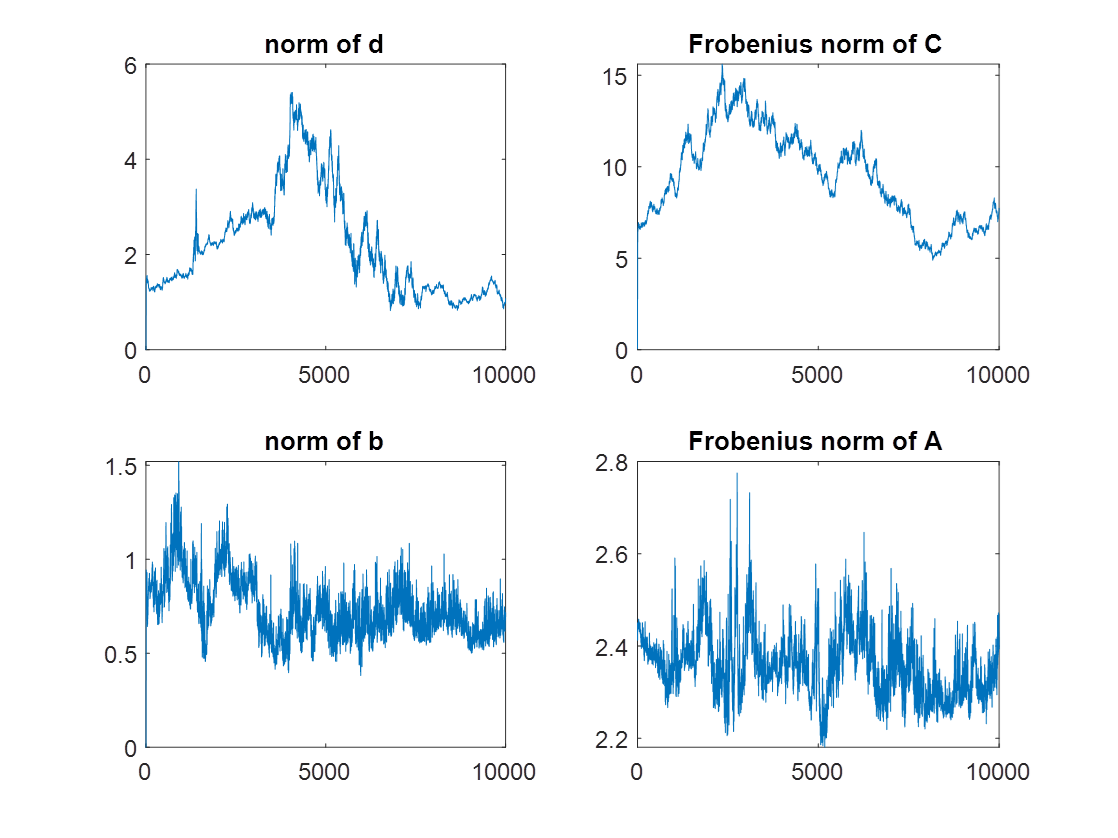
\includegraphics[width = .8\textwidth]{image030.png}
	\caption{(Frobenius) norm for \(\mathbf{d}\), \(\mathbf{C}\), \(\mathbf{b}\) and \(\mathbf{A}\)}
	\label{norms}
\end{figure}\\

It seems we may have not achieved stationary yet. And I show the average from iteration 8000 to 10000 as in Figure \ref{fig:LDS labeled revisit}

\begin{figure}[h!]
	\makebox[\linewidth][c]{%
		\centering
		\subfigure[overall mean firing rate]{\label{fig:a}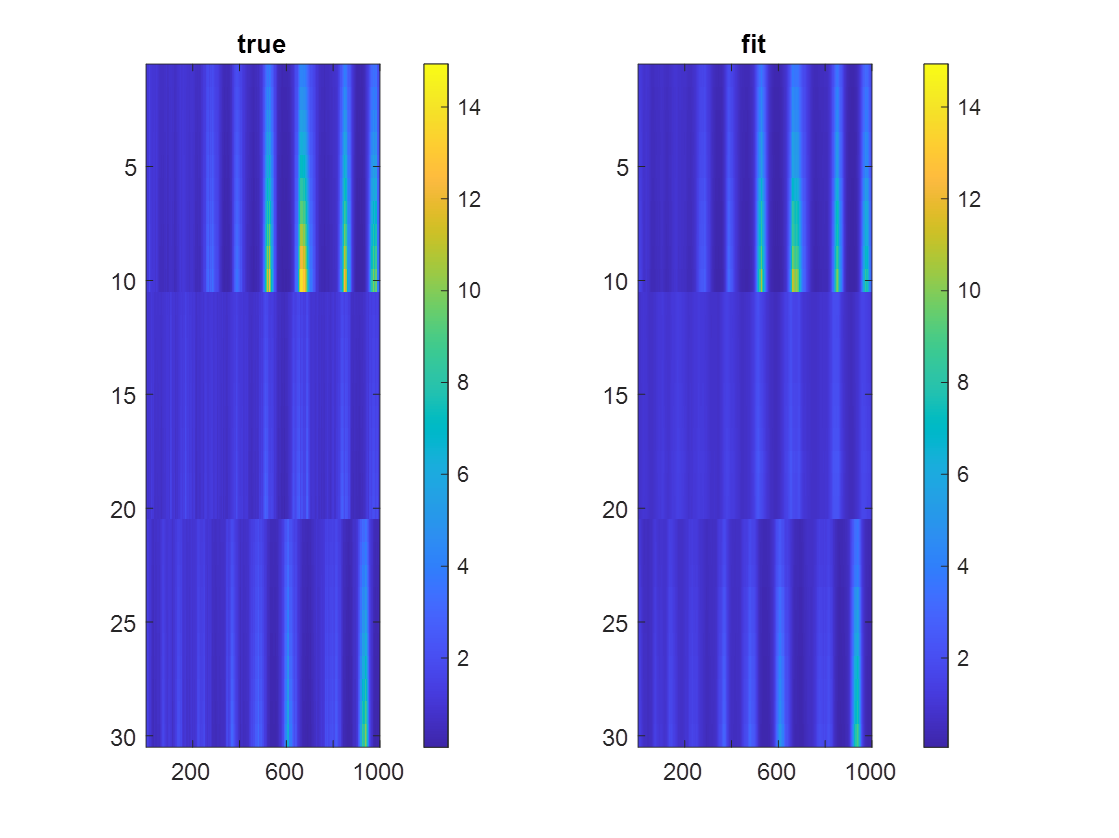
\includegraphics[width=0.55\textwidth]{image031.png}}%
		\subfigure[latents]{\label{fig:b}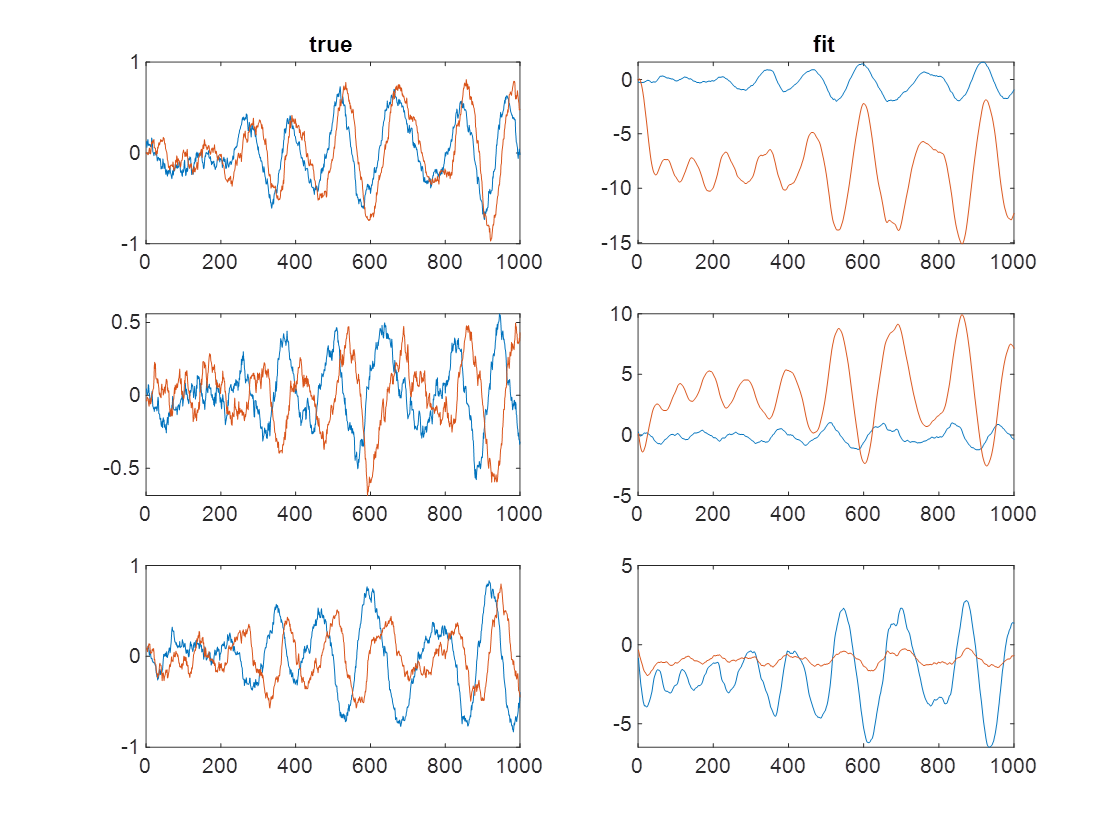
\includegraphics[width=0.55\textwidth]{image032.png}}%
		\subfigure[dynamics \(\mathbf{A}\)]{\label{fig:c}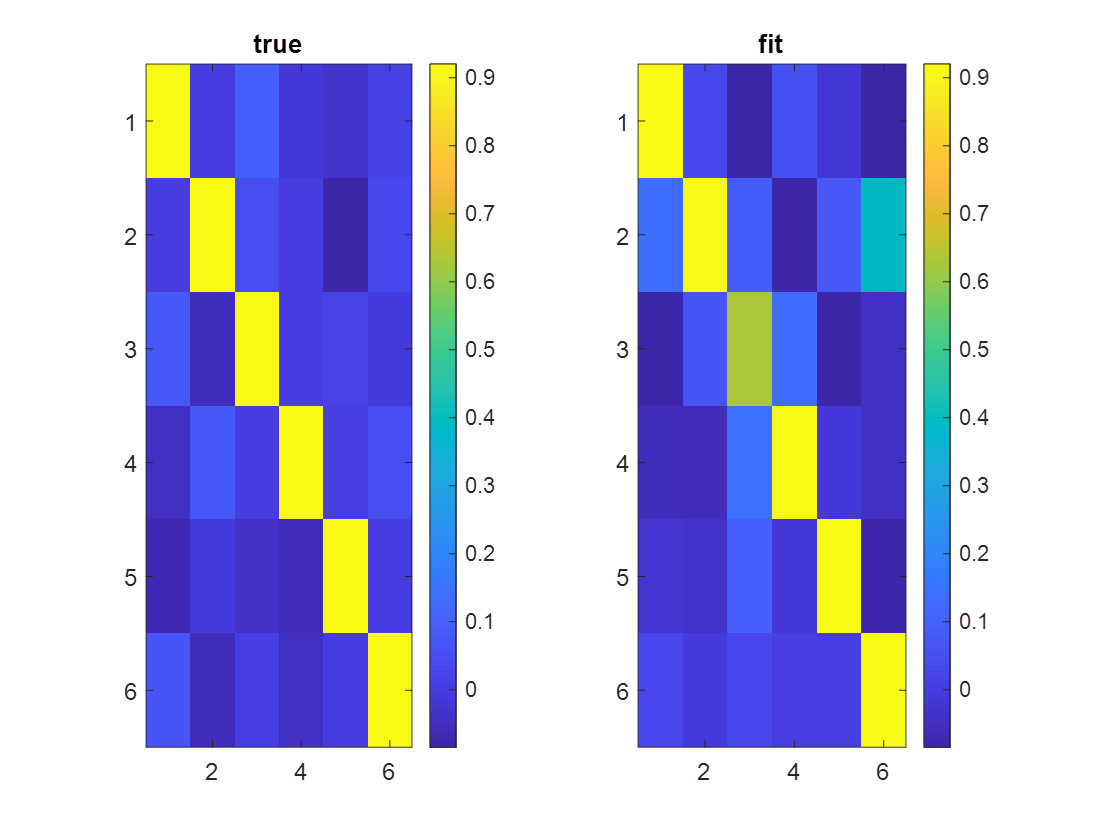
\includegraphics[width=0.55\textwidth]{image033.png}}%
	}
	\caption{LDS sample with labels}
	\label{fig:LDS labeled revisit}
\end{figure}

Things look much better! That means we need to improve the mixing of \(\mathbf{b}\) and \(\mathbf{A}\) later. (Also see if the mixing will be better for a more identifiable simulation)

\clearpage
\section{TODO}
\begin{enumerate}
	\def\labelenumi{(\arabic{enumi})}
	\item
	\textcolor{red}{\textbf{Do MV-GLM}}\\
	\item
	Check sampling trace and mixing.
	\item
	Find a more efficient way to generate new cluster parameters, otherwise the newly generated ones will always be rejected.
	\item
	improve DPMM. In current brute force implementation, the number of potential clusters can even go beyond number of neurons (\(N\)). There are several improvements, e.g. \href{https://link.springer.com/article/10.1007/s11222-009-9150-y}{Kalli et al., 2011}, \href{http://proceedings.mlr.press/v37/gea15.html}{Ge et al., 2015} and \href{https://link.springer.com/article/10.1007/s11222-014-9471-3}{Hastie et al, 2015}. Check them later.
	\item
	After all of them are resolved, switch to GP version
	
\end{enumerate}


\end{document}






